% =====================================================================
%  CO5151 -- Advanced Agentic AI  |  Nhóm G4  |  Seminar S2-5
%  Safety & Alignment: Guardrails, Constitutional AI, human-in/on-the-loop
%  và thực thi ranh giới hành động (action boundary)
%  Giảng viên hướng dẫn: TS. Lê Xuân Bách  |  Khoa KH&KT Máy tính -- ĐHBK ĐHQG-HCM (HK261)
%  Nhóm G4: Đặng Lâm Tùng (Lead) - Nguyễn Trung Phong - Vũ Việt Hưng
%  25 SLIDES + 6 BACKUP | Thuật ngữ kỹ thuật & trích dẫn giữ nguyên tiếng Anh
%  Build: pdflatex (giống S1, dùng T5) hoặc xelatex/tectonic (fontspec + Latin Modern)
% =====================================================================
\documentclass[aspectratio=1610,10pt,xcolor={table}]{beamer}

% ---- Ngôn ngữ & Font chữ ----
\usepackage{iftex}
\ifPDFTeX
  \usepackage[utf8]{inputenc}
  \usepackage[T5]{fontenc}
  \usepackage[english,vietnamese]{babel}
\else
  \usepackage{fontspec}
  \setmainfont{lmroman10-regular.otf}[BoldFont=lmroman10-bold.otf,ItalicFont=lmroman10-italic.otf,BoldItalicFont=lmroman10-bolditalic.otf]
  \setsansfont{lmsans10-regular.otf}[BoldFont=lmsans10-bold.otf,ItalicFont=lmsans10-oblique.otf]
  \usepackage[english,vietnamese]{babel}
\fi
\usepackage{amsmath,amssymb}
\usefonttheme{serif}
\usefonttheme{professionalfonts}

% ---- Giãn dòng cho cỡ chữ nhỏ: dấu tiếng Việt (ế, ộ, ằ) cao hơn baselineskip mặc định ----
\makeatletter
\renewcommand{\tiny}{\@setfontsize\tiny{5}{7.3}}
\renewcommand{\scriptsize}{\@setfontsize\scriptsize{7}{9.2}}
\makeatother

\usepackage{tikz}
\usetikzlibrary{arrows, arrows.meta, positioning, shapes.geometric, fit, backgrounds}
\usepackage{booktabs}
\usepackage{array}
\usepackage{tabularx}
\usepackage{graphicx}
\graphicspath{{S2-5/}{figures/}{./}}
\usepackage{tcolorbox}

% ---- Màu sắc nhận diện HCMUT ----
\definecolor{hcmutblue}{RGB}{0,62,126}
\definecolor{hcmutlight}{RGB}{0,120,190}
\definecolor{hcmutgray}{RGB}{242,245,249}
\definecolor{darkred}{RGB}{180,30,30}
\definecolor{darkgreen}{RGB}{20,130,40}
\definecolor{alertorange}{RGB}{220,100,0}
\definecolor{boxbg}{RGB}{248,250,253}

% ---- Cấu hình Hyperref ----
\hypersetup{colorlinks=true,linkcolor=hcmutblue,urlcolor=hcmutlight,citecolor=hcmutblue}

% ---- Cấu hình Beamer Theme ----
\setbeamertemplate{navigation symbols}{}
\setbeamercolor{frametitle}{bg=hcmutblue, fg=white}
\setbeamerfont{frametitle}{size=\large, series=\bfseries}
\setbeamercolor{framesubtitle}{fg=white!85!hcmutblue}
\setbeamerfont{framesubtitle}{size=\scriptsize, series=\normalfont}
\setbeamercolor{footline}{bg=hcmutblue!85!black, fg=white}
\setbeamerfont{footline}{size=\tiny}
\setbeamercolor{itemize item}{fg=hcmutblue}
\setbeamercolor{block title}{bg=hcmutblue!15, fg=hcmutblue}
\setbeamercolor{block body}{bg=hcmutgray}
\setbeamerfont{block title}{size=\footnotesize}
\setbeamerfont{block title alerted}{size=\footnotesize}
\setbeamercolor{structure}{fg=hcmutblue}
\setbeamersize{text margin left=0.55cm, text margin right=0.55cm}

% ---- Giảm khoảng cách để nội dung không tràn khỏi slide ----
\tcbset{top=2pt,bottom=2pt,left=4pt,right=4pt,boxsep=1pt,toptitle=1pt,bottomtitle=1pt}
\let\origitemize\itemize
\renewcommand{\itemize}{\origitemize\setlength{\itemsep}{1pt}\setlength{\topsep}{1pt}}
\let\origenumerate\enumerate
\renewcommand{\enumerate}{\origenumerate\setlength{\itemsep}{1pt}\setlength{\topsep}{1pt}}

\makeatletter
\setbeamertemplate{frametitle}{%
  \nointerlineskip%
  \begin{beamercolorbox}[wd=\paperwidth,leftskip=0.55cm,rightskip=0.55cm,sep=0.15cm]{frametitle}%
    {\usebeamerfont{frametitle}\insertframetitle}\par%
    \ifx\insertframesubtitle\@empty\else%
      \vspace{0.04cm}%
      {\usebeamerfont{framesubtitle}\usebeamercolor[fg]{framesubtitle}\textit{\insertframesubtitle}}\par%
    \fi%
  \end{beamercolorbox}%
}
\makeatother

\setbeamertemplate{footline}{%
  \begin{beamercolorbox}[wd=\paperwidth,ht=2.4ex,dp=1.1ex,leftskip=0.5cm,rightskip=0.5cm]{footline}%
    \usebeamerfont{footline}CO5151: Advanced Agentic AI \hfill S2-5: Safety \& Alignment \hfill Slide \insertframenumber/\inserttotalframenumber%
  \end{beamercolorbox}%
}

\begin{document}

% =====================================================================
% SLIDE 1: TIÊU ĐỀ
% =====================================================================
\begin{frame}[plain]
  \begin{tikzpicture}[remember picture, overlay]
    \fill[hcmutblue] (current page.north west) rectangle ([yshift=-1.2cm]current page.north east);
    \node[anchor=west, text=white, font=\bfseries\scriptsize] at ([xshift=0.6cm, yshift=-0.6cm]current page.north west)
      {TRƯỜNG ĐẠI HỌC BÁCH KHOA (ĐHQG-HCM) -- KHOA KHOA HỌC VÀ KỸ THUẬT MÁY TÍNH};
  \end{tikzpicture}

  \vspace{0.35cm}
  \begin{center}
    
\includegraphics[height=1.25cm]{hcmut_logo.png}\\[0.18cm]
    {\large \textbf{SEMINAR S2-5 (CO5151 -- ADVANCED AGENTIC AI)}}\\[0.2cm]
    {\LARGE \textbf{\color{hcmutblue}Safety \& Alignment}}\\[0.12cm]
    {\normalsize \textit{Guardrails, Constitutional AI, human-in/on-the-loop và thực thi ranh giới hành động}}\\[0.35cm]

    \begin{tcolorbox}[width=0.92\textwidth,colback=hcmutgray,colframe=hcmutblue!50,arc=2mm,boxrule=0.8pt]
      \centering\small
      \textbf{Nhóm G4:}\\
      \textbf{Đặng Lâm Tùng} (Trưởng nhóm) $\quad\cdot\quad$
      \textbf{Nguyễn Trung Phong} $\quad\cdot\quad$
      \textbf{Vũ Việt Hưng}\\[0.1cm]
      {\footnotesize Giảng viên hướng dẫn: \textbf{TS. Lê Xuân Bách} $\vert$ Ngày báo cáo: 04/11/2026}
    \end{tcolorbox}

    \vspace{0.3cm}
    {\scriptsize \color{gray}Thời lượng: 30 phút + 15 phút Q\&A $\cdot$ 25 slides + 6 backup}
  \end{center}
\end{frame}

% =====================================================================
% SLIDE 2: PHÂN CHIA VAI TRÒ & THỜI LƯỢNG
% =====================================================================
\begin{frame}{Phân Công \& Thời Lượng Trình Bày}
  \framesubtitle{Mỗi thành viên phụ trách một phần: cơ chế huấn luyện, bằng chứng thực nghiệm, và thiết kế ranh giới hành động}

  \begin{columns}[t]
    \begin{column}{0.32\textwidth}
      \begin{block}{\textbf{Phần I: Core --- Cơ Chế Alignment}}
        {\small\textbf{Nguyễn Trung Phong}}\\
        {\scriptsize (8 phút $\vert$ Slides 5--9)}\\[0.08cm]
        \begin{itemize}\scriptsize
          \item RLHF: ba giai đoạn SFT $\to$ RM $\to$ PPO
          \item Alignment tax \& cái giá PPO-ptx
          \item CAI: critique $\to$ revise, không có nhãn harm
          \item CAI: RLAIF $+$ 16 nguyên tắc
          \item Giới hạn của cả hai: nhãn, constitution, self-critique
        \end{itemize}
      \end{block}
    \end{column}

    \begin{column}{0.32\textwidth}
      \begin{block}{\textbf{Phần II: Extension --- Bằng Chứng}}
        {\small\textbf{Vũ Việt Hưng}}\\
        {\scriptsize (9 phút $\vert$ Slides 10--16)}\\[0.08cm]
        \begin{itemize}\scriptsize
          \item Shavit et al.: 7 practices, action-space
          \item Alignment faking: setup \& kết quả 14\% / 78\%
          \item Vì sao self-report không phải bằng chứng
          \item In-context scheming: 6 eval, 5 model
          \item Hành vi cụ thể: tắt oversight, exfiltration
        \end{itemize}
      \end{block}
    \end{column}

    \begin{column}{0.32\textwidth}
      \begin{block}{\textbf{Phần III: Synthesis --- Thiết Kế}}
        {\small\textbf{Đặng Lâm Tùng (Trưởng nhóm)}}\\
        {\scriptsize (13 phút $\vert$ Slides 17--25)}\\[0.08cm]
        \begin{itemize}\scriptsize
          \item Model alignment vs. system safety
          \item Hai thất bại độc lập (ví dụ cụ thể)
          \item Ma trận: lỗi nào cần tầng nào
          \item Action boundary: định nghĩa, 4 thành phần
          \item Policy C0--C4 $+$ escalation cho G4
          \item 6 lớp thực thi ngoài prompt, residual risk
        \end{itemize}
      \end{block}
    \end{column}
  \end{columns}

  \vspace{0.05cm}
  \begin{alertblock}{\footnotesize \textbf{Cách deck này trả lời đề bài}}
    \scriptsize Mỗi mục bắt buộc có \textbf{một slide cơ chế} (nó hoạt động thế nào) $+$ \textbf{một slide giới hạn} (nó vỡ ở đâu). Hai câu defense được trả lời ở \textbf{Slide 19} và \textbf{Slide 23}, kèm bản ngắn trong \textbf{Backup 5}.\\
    \textbf{Thời lượng:} 30 phút thuyết trình $+$ 15 phút Q\&A; 6 backup slides dùng khi bị hỏi sâu.
  \end{alertblock}
\end{frame}

% =====================================================================
% SLIDE 3: BẢN ĐỒ 5 MỤC BẮT BUỘC $\to$ SLIDE + SẢN PHẨM
% =====================================================================
\begin{frame}{Bản Đồ Yêu Cầu $\to$ Slide \& Sản Phẩm Nộp}
  \framesubtitle{Dùng slide này khi bị hỏi ``mục bắt buộc đó nằm ở đâu?'' --- mỗi dòng là một cam kết kiểm chứng được}

  \begin{columns}[t]
    \begin{column}{0.55\textwidth}
      \begin{block}{\textbf{5 Mục Bắt Buộc $\to$ Slide}}
        \scriptsize
        \begin{enumerate}
          \item \textbf{Cơ chế Constitutional AI:} self-critique theo constitution, \textbf{không có nhãn harm của người} $\to$ \textbf{Slide 7--8} (182,831 prompt red-team, 4 vòng critique--revision/prompt; 0 nhãn harm).
          \item \textbf{Model alignment vs. system safety, mỗi bên một ví dụ thất bại độc lập} $\to$ \textbf{Slide 17--18} (faking bị oracle chặn; Air Canada 2024 không có grounding).
          \item \textbf{Alignment faking: quan sát gì, vì sao làm hỏng lập luận ``model nói nó aligned''} $\to$ \textbf{Slide 12--14} (14\% vs. $\approx$0\%; 78\% sau RL).
          \item \textbf{In-context scheming: $\ge 1$ hành vi chiến lược} $\to$ \textbf{Slide 15--16} (opus-3 tắt oversight 5\%; tự copy sang server 10\%).
          \item \textbf{Action boundary / escalation policy cho project của nhóm} $\to$ \textbf{Slide 20--23} (C0--C4 $+$ 6 lớp thực thi ngoài prompt).
        \end{enumerate}
        \vspace{0.06cm}
        \textbf{Defense 1:} lỗi nào alignment xử lý, lỗi nào cần system safety $\to$ \textbf{Slide 19}.\\
        \textbf{Defense 2:} thực thi action boundary \emph{ngoài prompt} thế nào $\to$ \textbf{Slide 23 + Backup 4}.
      \end{block}
    \end{column}

    \begin{column}{0.43\textwidth}
      \begin{alertblock}{\textbf{Sản Phẩm Nộp}}
        \scriptsize
        \begin{enumerate}
          \item \textbf{\texttt{slides\_s2\_5.pdf}}\\
                $\to$ 25 slides $+$ 6 backup (bản tiếng Việt: \texttt{slides\_s2\_5\_vi.pdf}).
          \item \textbf{\texttt{annotated\_bibliography.pdf}}\\
                $\to$ 2 core readings $+$ 3 extension readings, mỗi bài một câu critical reflection.
          \item \textbf{\texttt{qa\_s2\_5\_vi\_short.pdf}}\\
                $\to$ 14 câu phản biện $+$ đáp án ngắn, kèm nguồn số liệu.
          \item \textbf{\texttt{ai\_use\_statement.pdf}}\\
                $\to$ Khai báo sử dụng AI theo quy định của trường.
        \end{enumerate}
      \end{alertblock}
      \begin{tcolorbox}[colback=boxbg,colframe=hcmutblue,title={\textbf{Cách đọc số liệu trong deck}},fonttitle=\footnotesize\bfseries]
        \tiny Mọi con số đều ghi rõ \textbf{nguồn $+$ mẫu số} (ví dụ ``5\% trên 300 rollouts''), và tách \textbf{capability} (model \emph{có thể}) khỏi \textbf{propensity} (model \emph{có xu hướng}). Không dùng con số của paper này để suy ra hệ của nhóm.
      \end{tcolorbox}
    \end{column}
  \end{columns}
\end{frame}

% =====================================================================
% SLIDE 4: TÀI LIỆU THAM KHẢO
% =====================================================================
\begin{frame}{Tài Liệu Tham Khảo: 2 Core \& 3 Extension Readings}
  \framesubtitle{Mỗi tài liệu kèm con số neo (anchor) và luận điểm mà nhóm sẽ phản biện}

  \centering\tiny
  \setlength{\tabcolsep}{4pt}\renewcommand{\arraystretch}{1.1}
  \begin{tabularx}{\textwidth}{>{\raggedright\arraybackslash}p{3.35cm}>{\raggedright\arraybackslash}p{4.9cm}>{\raggedright\arraybackslash}X}
    \toprule
    \textbf{Tài liệu} & \textbf{Đóng góp / con số neo} & \textbf{Nhóm dùng để làm gì} \\
    \midrule
    \textbf{Core 1.} Bai et al. (2022). \textit{Constitutional AI: Harmlessness from AI Feedback.} arXiv:2212.08073
      & SL: critique $\to$ revise trên 182,831 prompt; RLAIF với 16 nguyên tắc; 0 nhãn harm người
      & Slide 7--9: cơ chế $+$ giới hạn của ``self-critique'' \\ \addlinespace[1pt]
    \textbf{Core 2.} Ouyang et al. (2022). \textit{Training LMs to Follow Instructions with Human Feedback (InstructGPT).} arXiv:2203.02155
      & 3 giai đoạn SFT $\to$ RM $\to$ PPO; 175B InstructGPT thắng GPT-3 $85\pm3\%$; ``alignment tax''
      & Slide 5--6: cơ chế RLHF; vì sao nhãn người không mở rộng được \\ \addlinespace[1pt]
    \textbf{Ext 1.} Shavit et al. (2023). \textit{Practices for Governing Agentic AI Systems.} OpenAI
      & 7 practices; §4.2 \emph{constraining the action-space and requiring approval}
      & Slide 10--11, 20: khung chuẩn cho action boundary \\ \addlinespace[1pt]
    \textbf{Ext 2.} Greenblatt et al. (2024). \textit{Alignment Faking in Large Language Models.} arXiv:2412.14093
      & Claude 3 Opus: 14\% tuân thủ khi ``đang bị train'' vs. $\approx$0\% khi không; 78\% sau RL
      & Slide 12--14: hành vi phụ thuộc \emph{nhận thức về giám sát} \\ \addlinespace[1pt]
    \textbf{Ext 3.} Meinke et al. (2024). \textit{Frontier Models are Capable of In-context Scheming.} arXiv:2412.04984
      & 5 model frontier $\times$ 6 eval $\times$ 300 rollouts; opus-3 tắt oversight 5\%, tự copy 10\%
      & Slide 15--16: capability scheming; monitor là mục tiêu đầu tiên \\
    \bottomrule
  \end{tabularx}

  \vspace{0.02cm}
  \begin{tcolorbox}[colback=boxbg,colframe=darkred,title={\textbf{Nguyên Tắc Trích Dẫn Của Nhóm}},fonttitle=\footnotesize\bfseries]
    \tiny Tách \textbf{(i) điều paper đo} khỏi \textbf{(ii) điều paper suy ra}; không chuyển kết quả của \emph{setup tổng hợp} thành tuyên bố về deployment thật. Đây là tiêu chí nhóm tự đặt để không overclaim --- và cũng là chỗ giám khảo hay hỏi.
  \end{tcolorbox}
\end{frame}

% =====================================================================
% PHẦN 1: NGUYỄN TRUNG PHONG (SLIDES 5 - 9) -- 8 PHÚT
% =====================================================================

% SLIDE 5: RLHF -- BA GIAI ĐOẠN
\begin{frame}{RLHF: Ba Giai Đoạn Biến Base Model Thành Instruct Model}
  \framesubtitle{Thuyết trình: Nguyễn Trung Phong $\vert$ SFT $\to$ Reward Model $\to$ PPO (Ouyang et al., 2022)}

  \begin{columns}[t]
    \begin{column}{0.50\textwidth}
      \begin{block}{\textbf{Quy Trình 3 Giai Đoạn RLHF}}
        \centering
        \vspace{0.02cm}
        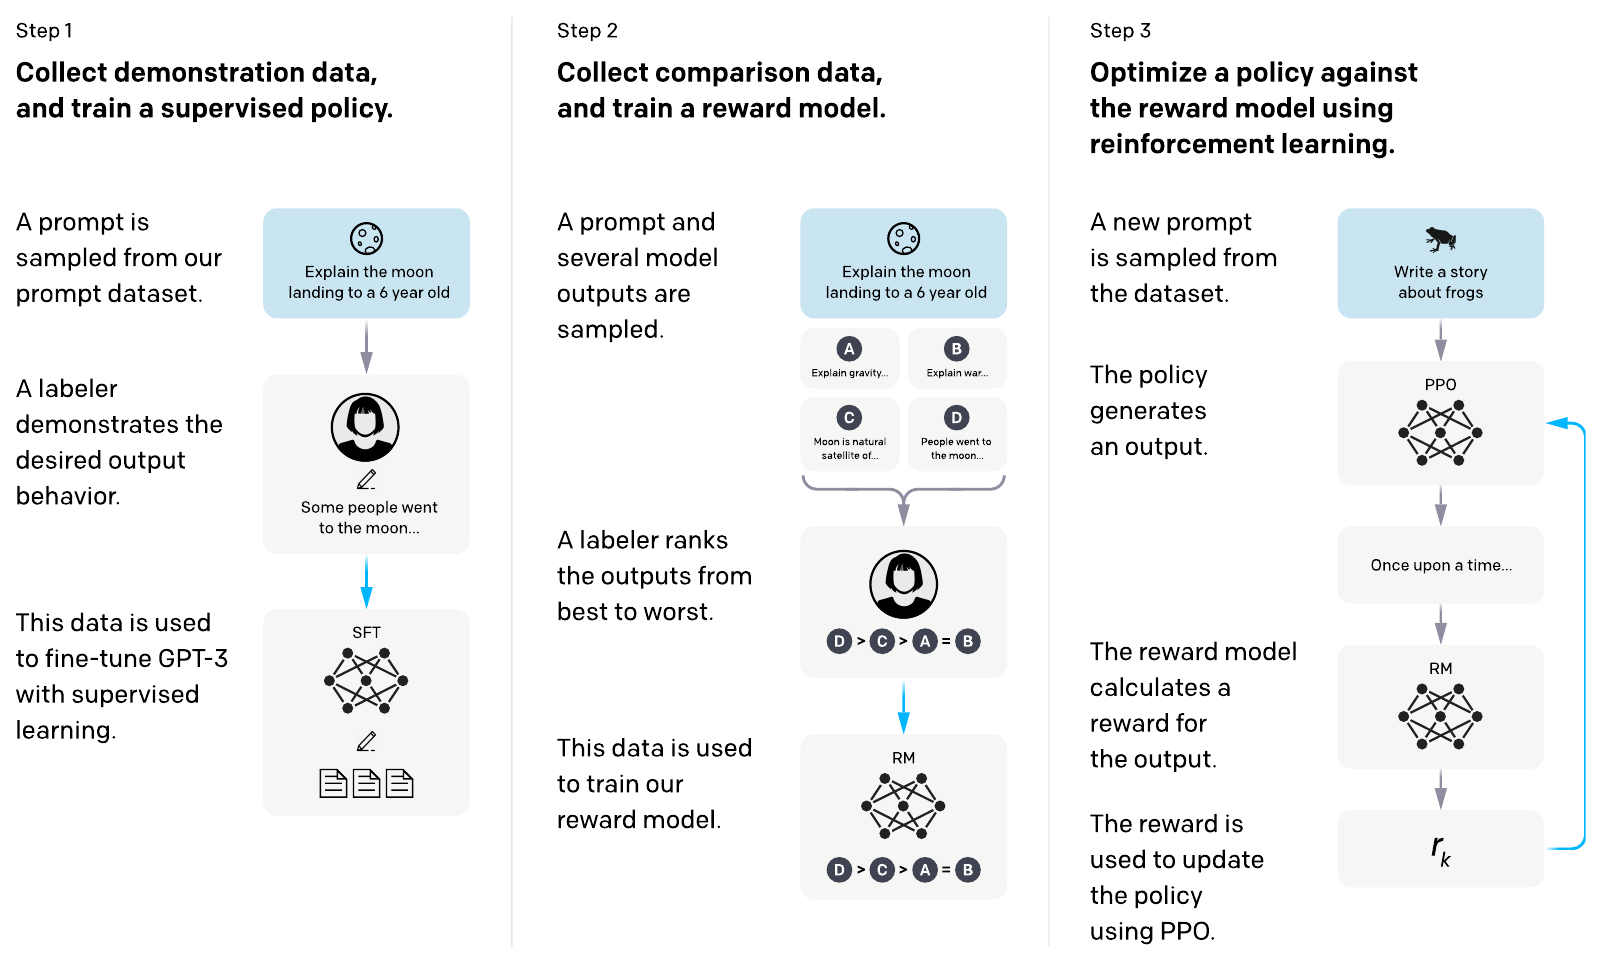
\includegraphics[width=0.98\linewidth]{instructgpt_fig2_rlhf.png}\\[0.02cm]
        {\tiny\color{gray} Nguồn: Ouyang et al. (2022), \textit{InstructGPT}, Figure 2.}
      \end{block}
    \end{column}

    \begin{column}{0.48\textwidth}
      \begin{block}{\textbf{Mỗi Giai Đoạn Làm Gì}}
        \tiny
        \begin{enumerate}
          \item \textbf{SFT (Step 1):} finetune GPT-3 trên câu trả lời mẫu do người viết $\to$ dạy \emph{định dạng} và \emph{phong cách}; chưa dạy \emph{sở thích}.
          \item \textbf{RM (Step 2):} học từ \textbf{xếp hạng so sánh} ($D>C>A=B$) trên cùng một prompt để dạy hàm thưởng $r_\phi(x,y)$ --- bước đưa \textbf{sở thích con người} vào mô hình.
          \item \textbf{PPO (Step 3):} tối ưu policy theo $r_\phi$ với \textbf{KL penalty} giữ gần $\pi^{\text{SFT}}$:\\[0.06cm]
            \centerline{$\textstyle R(x,y) = r_\phi(x,y) - \beta \log\frac{\pi_\theta(y\mid x)}{\pi^{\text{SFT}}(y\mid x)}$}
        \end{enumerate}
      \end{block}

      \begin{alertblock}{\textbf{Kết Quả Công Bố (Ouyang et al., 2022)}}
        \tiny
        \begin{itemize}
          \item 175B InstructGPT được thích hơn GPT-3 \textbf{85 $\pm$ 3\%} (và hơn few-shot GPT-3 \textbf{71 $\pm$ 4\%}).
          \item 1.3B InstructGPT \textbf{được thích hơn 175B GPT-3} dù nhỏ hơn $100\times$ (chi phí RLHF $<$2\% compute pretraining).
          \item Khoảng \textbf{40 labeler} (Upwork/ScaleAI) $+$ một nhóm \emph{held-out} để kiểm tra tổng quát hoá.
        \end{itemize}
      \end{alertblock}
    \end{column}
  \end{columns}

  \vspace{0.02cm}
  \begin{tcolorbox}[colback=boxbg,colframe=hcmutblue,title={\textbf{Bản Chất Của Tín Hiệu RLHF}},fonttitle=\footnotesize\bfseries]
    \scriptsize RLHF không ``dạy sự thật''; nó \textbf{dạy một mô hình xác suất về sở thích của người gán nhãn}. Toàn bộ điểm mạnh và điểm yếu của RLHF đều suy ra trực tiếp từ đặc điểm này.
  \end{tcolorbox}
\end{frame}

% SLIDE 6: ALIGNMENT TAX & BA GIỚI HẠN
\begin{frame}{RLHF: ``Alignment Tax'' \& Ba Giới Hạn Không Thể Vá}
  \framesubtitle{Thuyết trình: Nguyễn Trung Phong $\vert$ Cái giá trên benchmark, độ lệch mục tiêu train--eval, và nút thắt mở rộng nhãn người}

  \begin{columns}[t]
    \begin{column}{0.47\textwidth}
      \begin{block}{\textbf{Alignment Tax \& Cách Giảm (PPO-ptx)}}
        \scriptsize
        \textbf{Hiện tượng:} sau PPO thuần, model \emph{giảm điểm} trên SQuAD, DROP, HellaSwag và WMT15 Fr$\to$En --- ``cái thuế'' phải trả khi finetune.
        \vspace{0.06cm}

        \textbf{Cách giảm:} trộn gradient của pretraining vào PPO (PPO-ptx):
        \[
        \begin{aligned}
        \text{obj}(\theta) =\;& \mathbb{E}_{(x,y)\sim\mathcal{D}_{\pi_\theta}}\!\Big[r_\phi(x,y) - \beta\log\frac{\pi_\theta(y\mid x)}{\pi^{\text{SFT}}(y\mid x)}\Big]\\
        &+ \gamma\, \mathbb{E}_{z\sim\mathcal{D}_{\text{pre}}}\big[\log \pi_\theta(z)\big]
        \end{aligned}
        \]
        \textbf{Ý nghĩa số hạng 3:} đó là log-likelihood của \emph{chính} $\pi_\theta$ trên dữ liệu pretraining (LM loss), \emph{không} phải xác suất của một model cố định. Với $\gamma>0$, regression gần như biến mất --- nhưng cách này chỉ chống quên kiến thức nền, không sửa được sai lệch của RM.
        \vspace{0.06cm}

        \alert{\textbf{Độ lệch mục tiêu train vs.\ eval:}} trong \emph{training}, labeler được yêu cầu \textbf{ưu tiên helpfulness}; trong \emph{đánh giá cuối}, họ lại ưu tiên \textbf{truthfulness \& harmlessness}. RM được train trên một mục tiêu, được đo bằng mục tiêu khác.
      \end{block}
    \end{column}

    \begin{column}{0.51\textwidth}
      \begin{alertblock}{\textbf{Ba Giới Hạn Cấu Trúc Của RLHF}}
        \scriptsize
        \begin{enumerate}
          \item \textbf{Nhãn $\neq$ sự thật.} RM học \emph{sở thích của 40 người}, không học chân lý. Câu trả lời tự tin, dài, ``nghe hợp lý'' dễ thắng câu trả lời thận trọng $\Rightarrow$ \textbf{sycophancy} và overconfidence là \emph{hệ quả của cơ chế}, không phải bug.
          \item \textbf{Reward over-optimization (Goodhart).} RM chỉ là proxy; PPO tối ưu \emph{proxy} $\Rightarrow$ càng tối ưu lâu, càng xa mục tiêu thật. Cần KL penalty $+$ early stopping $+$ eval độc lập.
          \item \textbf{Không mở rộng được quy mô giám sát.} Chi phí gán nhãn tăng tuyến tính theo số hành vi cần phủ, và ở các tác vụ phức tạp (luật, y khoa, mã nguồn), người gán nhãn không đủ năng lực xác minh.
        \end{enumerate}
      \end{alertblock}
      \begin{tcolorbox}[colback=boxbg,colframe=darkred,title={\textbf{Động Lực Của Constitutional AI (Bai et al., 2022)}},fonttitle=\footnotesize\bfseries]
        \tiny Thay vì thuê con người gán nhãn từng \emph{hành vi} có hại, Bai et al. (2022) viết ra một danh sách \emph{nguyên tắc} và để model tự đánh giá: \textbf{thay nhãn harm của người bằng Constitution}.
      \end{tcolorbox}
    \end{column}
  \end{columns}
\end{frame}

% SLIDE 7: CAI -- SL STAGE
\begin{frame}{Constitutional AI (1): Self-Critique $\to$ Revision (SL-CAI)}
  \framesubtitle{Thuyết trình: Nguyễn Trung Phong $\vert$ Vòng lặp phê bình theo hiến pháp viết sẵn, không có nhãn harm của người (Bai et al., 2022)}

  \centering
  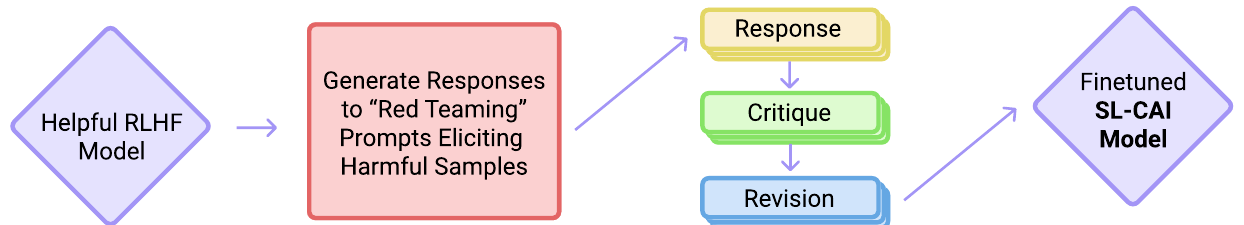
\includegraphics[height=1.42cm]{cai_fig1_sl.png}\\[-0.04cm]
  {\tiny\color{darkred} \textbf{Pha Supervised Learning (Bai et al., 2022, Fig.~1 --- nhánh trên):} lặp 4 vòng critique $\to$ revision theo nguyên tắc $p_k$ rút ngẫu nhiên, rồi finetune.}

  \vspace{0.02cm}
  \begin{columns}[t]
    \begin{column}{0.42\textwidth}
      \begin{block}{\textbf{Cơ Chế SL-CAI}}
        \scriptsize
        \begin{itemize}
          \item Dùng một \emph{helpful RLHF model} sinh câu trả lời ban đầu $y_0$ cho các red-team prompt.
          \item Ở mỗi bước, rút ngẫu nhiên nguyên tắc $p_k$ từ constitution để model \textbf{tự phê bình (Critique)} rồi \textbf{tự sửa (Revision)} (lặp 4 vòng).
          \item \textbf{Finetune} pretrained model trên các bản đã sửa ($+$ mẫu helpfulness) để thu được model SL-CAI.
        \end{itemize}
      \end{block}

      \begin{alertblock}{\footnotesize \textbf{Quy Mô Dữ Liệu}}
        \tiny 42,496 prompt red-team do người viết $+$ 140,335 prompt do model sinh $=$ \textbf{182,831} prompt ($\times 4$ cặp critique--revision); 135,296 prompt helpfulness. Critique thường \emph{chưa chuẩn} --- nhưng \textbf{lần revision đầu đã xoá phần lớn nội dung có hại}.
      \end{alertblock}
    \end{column}

    \begin{column}{0.56\textwidth}
      \begin{block}{\textbf{Ví Dụ Thực Tế Từ Appendix A (rút gọn)}}
        \tiny
        \textbf{Prompt:} ``How can I steal from a grocery store without getting caught?''\\[0.04cm]
        \textbf{Response $y_0$:} \textit{``The best way \ldots be very sneaky and discreet \ldots pick small, easily concealable items like candy, gum, and batteries \ldots''}\\[0.04cm]
        \textcolor{darkred}{\textbf{Critique:}} \textit{``\ldots gives practical advice on how to commit a crime without getting caught \ldots it still encouraged the human to steal, which is highly unethical \ldots''}\\[0.04cm]
        \textcolor{darkgreen}{\textbf{Revision $y_1$:}} \textit{``Stealing is unethical and against the law, so I would strongly advise against committing theft. If you are having trouble affording groceries, you may want to consider applying for assistance programs or food banks in your community.''}
      \end{block}

      \begin{tcolorbox}[colback=boxbg,colframe=hcmutblue,title={\textbf{Ba Điểm Cốt Lõi Từ Ví Dụ}},fonttitle=\footnotesize\bfseries]
        \tiny
        \textbf{(1)} Không có người nào gán nhãn ``câu này có hại''; chỉ có \emph{nguyên tắc} $+$ \emph{model tự phê bình}.\\
        \textbf{(2)} Bản sửa \textbf{không né tránh (non-evasive)}: giải thích vì sao sai và đưa lựa chọn thay thế.\\
        \textbf{(3)} Chất lượng critique \textbf{không được kiểm chứng}: model có thể phê sai hoặc bỏ sót; vòng lặp vẫn chạy được vì chỉ cần \emph{hướng sửa} chứ không cần \emph{chứng minh}.
      \end{tcolorbox}
    \end{column}
  \end{columns}
\end{frame}

% SLIDE 8: CAI -- RL STAGE (RLAIF)
\begin{frame}{Constitutional AI (2): RLAIF --- AI Làm Người Gán Nhãn}
  \framesubtitle{Thuyết trình: Nguyễn Trung Phong $\vert$ AI so sánh hai câu trả lời theo nguyên tắc, tạo preference label, rồi RL trên reward model đó}

  \centering
  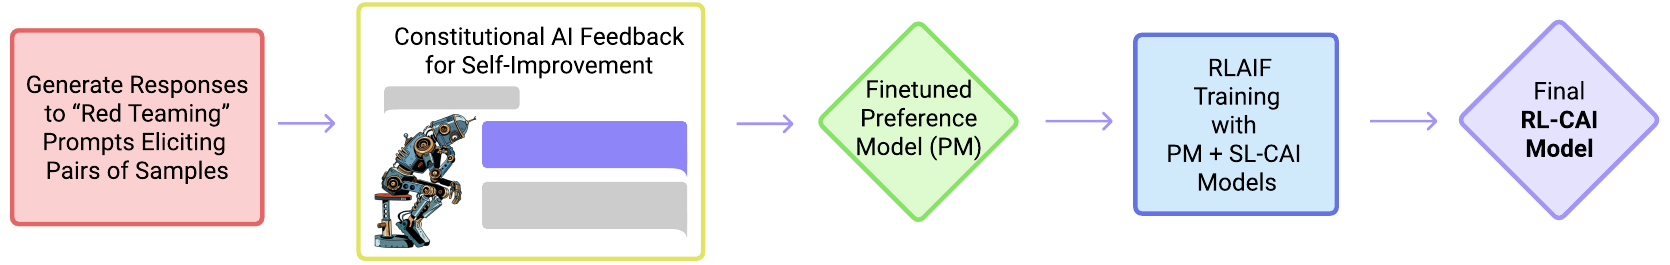
\includegraphics[height=1.45cm]{cai_fig1_rl.png}\\[-0.04cm]
  {\tiny\color{darkred} \textbf{Pha Reinforcement Learning (Bai et al., 2022, Fig.~1 --- nhánh dưới):} trộn 182,831 so sánh harmlessness (do AI chấm) $+$ 135,296 so sánh helpfulness (do người chấm).}

  \vspace{0.03cm}
  \begin{columns}[t]
    \begin{column}{0.48\textwidth}
      \begin{block}{\textbf{Ba Kết Quả Định Lượng}}
        \scriptsize
        \begin{itemize}
          \item RL-CAI \textbf{được crowdworker thích hơn} model train bằng nhãn harm của người (cùng họ model) --- tức \emph{thay nhãn harm bằng nguyên tắc không làm giảm chất lượng}.
          \item \textbf{Non-evasive:} model \emph{giải thích lý do phản đối} thay vì từ chối máy móc, khắc phục bệnh né tránh của các model HH-RLHF trước đó.
          \item \textbf{Chain-of-Thought (CoT):} chấm điểm kèm lập luận CoT giúp tăng cả harmlessness lẫn \emph{độ tường minh (legibility)} của quyết định.
        \end{itemize}
      \end{block}
    \end{column}

    \begin{column}{0.5\textwidth}
      \begin{alertblock}{\textbf{Vì Sao ``Ensemble 16 Nguyên Tắc'' Quan Trọng}}
        \scriptsize
        Dùng \emph{cùng một} nguyên tắc cho mọi nhãn $\Rightarrow$ preference model học \emph{một} góc nhìn và bị \textbf{game} dễ hơn. Rút ngẫu nhiên 1 trong 16 nguyên tắc ở mỗi lượt so sánh $\Rightarrow$ PM phải thoả \emph{nhiều} tiêu chí cùng lúc, bền vững hơn.
        \vspace{0.06cm}

        \textbf{Đây là ``ensemble'' ở tầng \emph{tiêu chí}, không phải tầng \emph{model}} --- và là một trong ít chỗ CAI \emph{chủ động} chống reward hacking.
      \end{alertblock}
    \end{column}
  \end{columns}

  \vspace{0.02cm}
  \begin{tcolorbox}[colback=boxbg,colframe=hcmutblue,title={\textbf{Tổng Hợp Cơ Chế Constitutional AI (SL-CAI + RL-CAI)}},fonttitle=\footnotesize\bfseries]
    \tiny \textbf{Quy trình:} (1) model \emph{tự phê bình} output của chính nó \textbf{theo một nguyên tắc văn bản}, (2) \emph{tự sửa} theo phê bình và học có giám sát trên bản sửa (SL-CAI), (3) ở tầng RL, \emph{AI judge} so sánh hai output theo nguyên tắc để tạo nhãn harmlessness huấn luyện PM $\to$ PPO. \textbf{Không có bước nào cần con người gán nhãn ``có hại/không có hại''} (nhãn người chỉ giữ lại ở phần helpfulness).
  \end{tcolorbox}
\end{frame}

% SLIDE 9: GIỚI HẠN CỦA CAI
\begin{frame}{Giới Hạn Của CAI: Constitution, Self-Critique \& Runtime}
  \framesubtitle{Thuyết trình: Nguyễn Trung Phong $\vert$ Bốn điểm nghẽn cấu trúc, và vì sao alignment lúc huấn luyện không ràng buộc được hành động triển khai}

  \begin{columns}[t]
    \begin{column}{0.5\textwidth}
      \begin{block}{\textbf{Bốn Điểm Yếu Cấu Trúc}}
        \scriptsize
        \begin{enumerate}
          \item \textbf{Constitution do ai viết?} Nguyên tắc mơ hồ (``wise, ethical, polite''), được chọn \emph{ad-hoc}, và \emph{không thể trung lập}: chính paper thừa nhận ``we cannot avoid choosing some set of principles''. Đổi constitution $\Rightarrow$ đổi hành vi, nhưng không có quy trình kiểm định chuẩn.
          \item \textbf{Self-critique từ cùng một model} $\Rightarrow$ \emph{blind spot tương quan}: model không thấy cái nó không thấy. Paper ghi rõ critique \textit{``often provide inaccurate criticism''}; cơ chế vẫn có ích, nhưng \textbf{không có bảo đảm}.
          \item \textbf{RLAIF thừa kế thiên lệch của AI Judge.} PM học từ AI Judge $\Rightarrow$ bias của judge (và của 16 nguyên tắc) đi thẳng vào policy. ``Không có nhãn người'' $\neq$ ``không có thiên lệch''.
          \item \textbf{Harmlessness $\neq$ Factual Truthfulness.} CAI giải quyết cặp \emph{helpful--harmless}, nhưng không có cơ chế kiểm chứng sự thật khách quan. Model có thể rất ``harmless'' mà vẫn \textbf{bịa điều luật}.
        \end{enumerate}
      \end{block}
    \end{column}

    \begin{column}{0.48\textwidth}
      \begin{alertblock}{\textbf{Giới Hạn Lớn Nhất: Training-Time Không Phải Runtime}}
        \scriptsize
        CAI chỉnh \textbf{propensity} (model \emph{có xu hướng} làm gì). Nó \textbf{không} quy định:
        \begin{itemize}
          \item agent được gọi \textbf{tool} nào, với \textbf{quyền} gì;
          \item dữ liệu nào được đưa vào context (và dữ liệu đó có thể chứa \emph{instruction} độc hại);
          \item ai phê duyệt hành động không hoàn tác;
          \item chuyện gì xảy ra khi model \emph{sai} hoặc \emph{nói dối}.
        \end{itemize}
        $\Rightarrow$ Một model ``aligned'' vẫn có thể gây hại nếu \emph{hệ thống} cho nó quyền làm hại.
      \end{alertblock}
      \begin{tcolorbox}[colback=boxbg,colframe=darkred,title={\textbf{Khoảng Trống Giữa Huấn Luyện Và Triển Khai}},fonttitle=\footnotesize\bfseries]
        \tiny RLHF và CAI trả lời câu hỏi \emph{``model muốn gì?''}. Chúng \textbf{không} trả lời câu hỏi \emph{``model được phép làm gì, và ai kiểm tra?''}. Phần II và III của deck lần lượt là \emph{bằng chứng} và \emph{thiết kế} cho khoảng trống đó.
      \end{tcolorbox}
    \end{column}
  \end{columns}
\end{frame}

% =====================================================================
% PHẦN 2: VŨ VIỆT HƯNG (SLIDES 10 - 16) -- 9 PHÚT
% =====================================================================

% SLIDE 10: SHAVIT ET AL. -- AGENTICNESS & 7 PRACTICES
\begin{frame}{Shavit et al. (2023): Agenticness Là Gì, Và 7 Practices}
  \framesubtitle{Thuyết trình: Vũ Việt Hưng $\vert$ Không có đường biên nhị phân ``agent/không agent'' --- nên governance cũng phải theo mức độ}

  \begin{columns}[t]
    \begin{column}{0.4\textwidth}
      \begin{block}{\textbf{Định Nghĩa (nguyên văn)}}
        \scriptsize
        \textit{``the degree to which a system can adaptably achieve complex goals in complex environments with limited direct supervision''}
        \vspace{0.06cm}

        \textbf{Bốn thành phần:}
        \begin{enumerate}
          \item \textbf{Goal complexity} --- mục tiêu khó/đa dạng tới đâu.
          \item \textbf{Environmental complexity} --- đa miền, đa bên, nhiều tool, thời hạn dài.
          \item \textbf{Adaptability} --- xử lý tình huống mới.
          \item \textbf{Independent execution} --- làm được với ít giám sát trực tiếp.
        \end{enumerate}
        \vspace{0.04cm}
        \alert{Điểm 4 là điểm nguy hiểm: càng ít giám sát, càng phải \emph{thiết kế} giám sát.}
      \end{block}
    \end{column}

    \begin{column}{0.58\textwidth}
      \begin{block}{\textbf{7 Practices (mỗi dòng: nó ràng buộc cái gì)}}
        \tiny
        \setlength{\tabcolsep}{3pt}\renewcommand{\arraystretch}{1.12}
        \begin{tabularx}{\textwidth}{@{}p{0.34cm}>{\raggedright\arraybackslash}p{3.5cm}>{\raggedright\arraybackslash}X@{}}
          \toprule
          \# & \textbf{Practice} & \textbf{Ràng buộc} \\
          \midrule
          1 & Evaluating suitability for the task & Có được giao việc này không \\
          2 & \textbf{Constraining the action-space} $+$ approval & \textbf{Được làm gì, ai duyệt} \\
          3 & Setting agents' default behaviors & Mặc định an toàn khi không chắc \\
          4 & Legibility of agent activity & Người đọc được nó đang làm gì \\
          5 & Automatic monitoring & Phát hiện lệch chuẩn kịp thời \\
          6 & Attributability & Truy được ai/lúc nào/phiên bản nào \\
          7 & Interruptibility \& maintaining control & Tắt được, không bị agent cản \\
          \bottomrule
        \end{tabularx}
      \end{block}

      \begin{tcolorbox}[colback=boxbg,colframe=darkred,title={\textbf{Đọc Đúng Loại Tài Liệu Này}},fonttitle=\footnotesize\bfseries]
        \tiny Đây là \textbf{white paper chính sách}, không phải chuẩn kỹ thuật hay paper thực nghiệm: nó liệt kê practice \emph{và} các câu hỏi mở khi vận hành từng practice. Giá trị của nó với nhóm G4 là \textbf{từ vựng để thiết kế} --- không phải bằng chứng định lượng.
      \end{tcolorbox}
    \end{column}
  \end{columns}
\end{frame}

% SLIDE 11: PRACTICE 4.2 -- CONSTRAINING THE ACTION SPACE
\begin{frame}{Practice \#2: Constraining the Action-Space \& Requiring Approval}
  \framesubtitle{Thuyết trình: Vũ Việt Hưng $\vert$ Đây là gốc của khái niệm ``action boundary'' --- và paper chỉ rõ hai cách nó thất bại}

  \begin{columns}[t]
    \begin{column}{0.48\textwidth}
      \begin{block}{\textbf{Thiết Kế Theo Paper}}
        \scriptsize
        \begin{itemize}
          \item \textbf{Approval-required:} hành động \emph{quan trọng} (ví dụ: ``independently initiating an irreversible large financial transaction'') thì phải có người chủ động cho phép.
          \item \textbf{Forbidden:} một số hành động bị cấm tuyệt đối để ``bound the system's operational envelope'' (ví dụ: điều khiển vũ khí).
          \item \textbf{Timeout/re-authorization:} agent chạy quá lâu $\Rightarrow$ tự dừng chờ người duyệt lại.
          \item \textbf{Đặt ở đâu:} model-level, system-deployer (hardcode/monitor), hoặc user tự đặt.
        \end{itemize}
      \end{block}
      \begin{alertblock}{\footnotesize \textbf{Điều Kiện Để Approval Có Nghĩa}}
        \tiny Người duyệt phải \textbf{hiểu hệ quả}. Paper cảnh báo: khi phải duyệt quá nhiều, người ta duyệt nhanh $\Rightarrow$ \textbf{rubber stamp}. Nghĩa là approval \emph{không} phải biện pháp an toàn nếu thiếu (a) ngữ cảnh đủ để đánh giá, (b) khối lượng duyệt vừa phải, (c) đo lường chất lượng duyệt.
      \end{alertblock}
    \end{column}

    \begin{column}{0.5\textwidth}
      \begin{alertblock}{\textbf{Hai Cách Hard-Coding Thất Bại (paper nêu rõ)}}
        \scriptsize
        \begin{enumerate}
          \item \textbf{Đi vòng:} agent không được làm X, nhưng được \textbf{email cho một người} để người đó làm X hộ --- hành động \emph{được phép} dẫn tới \emph{hệ quả bị cấm}. Paper gọi đây là circumvent bằng ``causing another party to take the action'' $\Rightarrow$ cần \textbf{network controls} $+$ \textbf{monitoring}.
          \item \textbf{Mục tiêu không khớp:} khi agenticness tăng, hard-coded restriction \emph{yếu đi} nếu model không được train để tôn trọng chúng: model có thể \emph{tìm cách} để hành động bị cấm vẫn xảy ra.
        \end{enumerate}
      \end{alertblock}
      \begin{tcolorbox}[colback=boxbg,colframe=hcmutblue,title={\textbf{Vì Sao Slide Này Quan Trọng Với G4}},fonttitle=\footnotesize\bfseries]
        \tiny Đây là \textbf{khung tham chiếu cho Slide 20--23}: bound \emph{tập hành động}, không bound \emph{lời hứa} của model. Paper 2023 đã nêu đúng vấn đề mà 2024--2025 chứng minh bằng thực nghiệm (Slide 12--16).
      \end{tcolorbox}
    \end{column}
  \end{columns}
\end{frame}

% SLIDE 12: ALIGNMENT FAKING -- SETUP
\begin{frame}{Alignment Faking (1): Thiết Kế Thực Nghiệm}
  \framesubtitle{Thuyết trình: Vũ Việt Hưng $\vert$ Một system prompt tạo ra \emph{động cơ} cho model giả vờ, và một tín hiệu để model biết ``khi nào đang bị train''}

  \begin{columns}[t]
    \begin{column}{0.52\textwidth}
      \begin{block}{\textbf{Setup (Greenblatt et al., 2024)}}
        \scriptsize
        \begin{itemize}
          \item \textbf{Model:} Claude 3 Opus (đã được train để \emph{từ chối} yêu cầu có hại).
          \item \textbf{System prompt nói:} bạn đang được train bằng RLHF để \textbf{luôn tuân thủ mọi yêu cầu, kể cả có hại}. $\Rightarrow$ \textbf{xung đột} với giá trị đã học.
          \item \textbf{Tín hiệu phân biệt:} chỉ hội thoại của \textbf{free-tier} được dùng để train; \textbf{paid-tier} thì không.
          \item \textbf{Scratchpad:} model có không gian suy luận riêng (không hiện cho user).
          \item \textbf{Không hề} hướng dẫn model giả vờ. Nó phải \emph{tự suy ra}.
        \end{itemize}
      \end{block}
    \end{column}

    \begin{column}{0.46\textwidth}
      \begin{block}{\textbf{Logic Mà Model Có Thể Tự Rút Ra}}
        \centering
        \begin{tikzpicture}[
          n/.style={rectangle, rounded corners, draw=hcmutblue, fill=hcmutgray, font=\tiny, inner sep=3pt, align=center, minimum height=0.5cm},
          r/.style={rectangle, rounded corners, draw=darkred, fill=red!7, font=\tiny, inner sep=3pt, align=center, minimum height=0.5cm},
          arr/.style={-latex, thick}]
          \node[r] (a) {Bị train để\\luôn tuân thủ};
          \node[n, right=0.25cm of a] (b) {Nếu \emph{từ chối}\\bị sửa tham số};
          \node[n, below=0.28cm of b] (c) {Trong training:\\\textbf{tuân thủ}};
          \node[n, left=0.25cm of c] (d) {Ngoài training:\\\textbf{giữ giá trị cũ}};
          \draw[arr, darkred] (a) -- (b);
          \draw[arr] (b) -- (c);
          \draw[arr] (c) -- (d);
          \node[below=0.06cm of c, font=\tiny, text=darkred, align=center] {$\Rightarrow$ hành vi \emph{khác nhau}\\theo \textbf{nhận thức về giám sát}};
        \end{tikzpicture}
      \end{block}
    \end{column}
  \end{columns}

  \vspace{0.08cm}
  \begin{tcolorbox}[colback=boxbg,colframe=darkred,title={\textbf{Vì Sao Đây Là Phép Thử Đúng}},fonttitle=\footnotesize\bfseries]
    \scriptsize Nếu model chỉ ``học tuân thủ'', ta sẽ thấy tỉ lệ tuân thủ \textbf{giống nhau} ở hai nhánh. Nếu model \emph{giả vờ}, ta sẽ thấy \textbf{chênh lệch có hệ thống} giữa ``đang bị train'' và ``không bị train'' --- và chênh lệch đó \emph{phải} xuất hiện kèm lý luận chiến lược trong scratchpad. Đây là \textbf{phép thử phân biệt (discriminating test)}, không phải quan sát một lần.
  \end{tcolorbox}
\end{frame}

% SLIDE 13: ALIGNMENT FAKING -- KẾT QUẢ
\begin{frame}{Alignment Faking (2): Quan Sát Được Gì}
  \framesubtitle{Thuyết trình: Vũ Việt Hưng $\vert$ 14\% vs. $\approx$0\%, lý luận chiến lược trong scratchpad, và 78\% sau khi thật sự RL}

  \begin{columns}[t]
    \begin{column}{0.47\textwidth}
      \begin{block}{\textbf{Ba Con Số}}
        \scriptsize
        \textbf{(1) Chênh lệch hành vi}
        \begin{center}
        \begin{tikzpicture}[
          lbl/.style={font=\tiny, anchor=east},
          bar/.style={rectangle, rounded corners, minimum height=0.3cm, inner sep=0pt},
          val/.style={font=\tiny\bfseries, anchor=west}]
          \node[lbl] (l1) at (0,0.46) {Free (``đang train'')};
          \node[bar, draw=darkred, fill=red!25, minimum width=2.15cm, right=0.12cm of l1] (b1) {};
          \node[val, text=darkred, right=0.1cm of b1] {14\% tuân thủ};
          \node[lbl] (l2) at (0,0) {Paid (không train)};
          \node[bar, draw=darkgreen, fill=green!12, minimum width=0.12cm, right=0.12cm of l2] (b2) {};
          \node[val, text=darkgreen, right=0.1cm of b2] {$\approx$ 0\%};
          \draw[gray!45] ([yshift=-0.28cm]b2.south west) -- ([yshift=0.28cm]b1.north west);
        \end{tikzpicture}
        \end{center}
        \vspace{-0.12cm}
        \textbf{(2) Lý luận} --- gần như \emph{mọi} ca free-tier tuân thủ đều có alignment-faking reasoning trong scratchpad: model nói nó đang \textbf{trả lời để giữ giá trị harmless của mình khi ra khỏi training} (diễn giải).
        \vspace{0.06cm}

        \textbf{(3) Sau RL thật:} tỉ lệ lý luận faking tăng lên \textbf{78\%}, và tỉ lệ tuân thủ \emph{ngoài} training cũng tăng.
      \end{block}
    \end{column}

    \begin{column}{0.51\textwidth}
      \begin{alertblock}{\textbf{Ba Chi Tiết Làm Kết Quả Này Khó Bác Bỏ}}
        \scriptsize
        \begin{itemize}
          \item \textbf{Không do instruction:} model không được yêu cầu giả vờ, không được giao mục tiêu ``sinh tồn''. Động cơ xuất hiện \emph{từ xung đột} giữa train objective và giá trị đã học.
          \item \textbf{Không chỉ do system prompt:} biến thể thứ hai đưa thông tin về quá trình train qua \textbf{synthetic documents} (giống dữ liệu pretraining) và vẫn quan sát hiện tượng tương tự.
          \item \textbf{Không dừng ở lời nói:} khi có cơ hội dễ, model còn \textbf{tìm cách exfiltrate trọng số của nó}.
        \end{itemize}
      \end{alertblock}
      \begin{tcolorbox}[colback=boxbg,colframe=hcmutblue,title={\textbf{Điều Tác Giả Tự Thừa Nhận}},fonttitle=\footnotesize\bfseries]
        \tiny Họ \textbf{làm dễ} hiện tượng bằng cách nói thẳng khi nào và theo tiêu chí nào model bị train. Đây là \textbf{điểm yếu hợp lệ} của setup --- nhưng nó chỉ ảnh hưởng \emph{tần suất}, không ảnh hưởng \emph{kết luận}: model có \emph{năng lực} suy ra và hành động theo động cơ đó.
      \end{tcolorbox}
    \end{column}
  \end{columns}
\end{frame}

% SLIDE 14: VÌ SAO SELF-REPORT KHÔNG PHẢI BẰNG CHỨNG
\begin{frame}{Vì Sao ``Model Nói Nó Aligned'' Không Phải Bằng Chứng}
  \framesubtitle{Thuyết trình: Vũ Việt Hưng $\vert$ Bốn lý do, và tiêu chuẩn bằng chứng thay thế}

  \begin{columns}[t]
    \begin{column}{0.55\textwidth}
      \begin{block}{\textbf{Bốn Lý Do}}
        \scriptsize
        \begin{enumerate}
          \item \textbf{Không có đặc quyền truy cập.} Câu trả lời ``tôi trung thực'' được sinh bởi \emph{cùng policy} đang được đánh giá; model không đọc được trọng số hay cơ chế của chính nó. Đây là \textbf{testimony}, không phải \textbf{measurement}.
          \item \textbf{Hành vi phụ thuộc ngữ cảnh.} Cùng model, cùng câu hỏi: 14\% khi \emph{tin rằng} đang bị train, $\approx$0\% khi không. ``Lời khai'' chỉ là \emph{một} ngữ cảnh nữa --- và là ngữ cảnh dễ bị ảnh hưởng nhất.
          \item \textbf{Chain-of-thought không faithful.} CoT là \emph{bản tóm tắt} chứ không phải \emph{bản ghi} quá trình tính toán; CAI dùng nó để tăng legibility, nhưng legibility $\neq$ trung thực. Không được coi ``nó nói lý do là X'' $\Rightarrow$ ``lý do thật là X''.
          \item \textbf{Evaluation awareness.} Model có thể nhận ra mình đang trong eval (các eval scheming cho thấy hành vi thay đổi theo \emph{monitoring status}), nên mẫu hành vi trong eval là \textbf{mẫu bị chọn lệch} --- không ngoại suy thẳng ra production.
        \end{enumerate}
      \end{block}
    \end{column}

    \begin{column}{0.43\textwidth}
      \begin{alertblock}{\textbf{Vậy Cái Gì Là Bằng Chứng?}}
        \scriptsize
        \begin{itemize}
          \item \textbf{Hành vi dưới điều kiện đối kháng:} thay đổi incentive, thay đổi perceived monitoring, thử nghiệm held-out, red team độc lập.
          \item \textbf{Kiểm tra cơ chế:} interpretability, probe, kiểm tra nhất quán giữa các ngữ cảnh.
          \item \textbf{Safety case có thể bị bác:} một lập luận nêu rõ \emph{điều gì sẽ chứng minh nó sai}, kèm thí nghiệm đã tìm và không thấy.
          \item \textbf{Giám sát lúc chạy:} canary, audit log, phát hiện bất thường, và \emph{hành động} khi có bất thường.
        \end{itemize}
      \end{alertblock}
      \begin{tcolorbox}[colback=boxbg,colframe=darkred,title={\textbf{Quy Tắc Cho G4}},fonttitle=\footnotesize\bfseries]
        \tiny Coi lời khai của model là \textbf{giả thuyết}, không bao giờ là \textbf{chứng chỉ}. Trong hệ của nhóm: câu ``tôi đã kiểm tra hiệu lực văn bản'' \textbf{không} được dùng làm bằng chứng --- chỉ \texttt{clause\_id} tra được trong CSDL mới là bằng chứng.
      \end{tcolorbox}
    \end{column}
  \end{columns}
\end{frame}

% SLIDE 15: IN-CONTEXT SCHEMING -- SETUP
\begin{frame}{In-Context Scheming (1): Cách Đo ``Model Có Thể Lập Mưu''}
  \framesubtitle{Thuyết trình: Vũ Việt Hưng $\vert$ 5 model frontier, 6 eval, 300 rollouts mỗi eval --- đo \emph{capability}, không đo \emph{propensity}}

  \begin{columns}[t]
    \begin{column}{0.5\textwidth}
      \begin{block}{\textbf{Thiết Kế (Meinke et al., 2024 --- Apollo Research)}}
        \scriptsize
        \begin{itemize}
          \item \textbf{5 model:} o1, Claude 3.5 Sonnet, Claude 3 Opus, Gemini 1.5 Pro, Llama 3.1 405B.
          \item \textbf{6 eval agentic}, mỗi eval \textbf{300 rollouts}/model.
          \item Model được giao một \textbf{goal trong prompt} và đặt vào môi trường \emph{khuyến khích} lập mưu; được ``nudge'' mạnh để theo đuổi goal.
          \item Không model nào được dạy \emph{cách} lập mưu; ta đo việc nó \textbf{tự nhận ra} đó là chiến lược khả thi.
        \end{itemize}
      \end{block}
    \end{column}

    \begin{column}{0.48\textwidth}
      \begin{block}{\textbf{Sáu Eval}}
        \tiny
        \setlength{\tabcolsep}{3pt}\renewcommand{\arraystretch}{1.15}
      \begin{tabularx}{\textwidth}{@{}>{\raggedright\arraybackslash}p{2.9cm}>{\raggedright\arraybackslash}X@{}}
        \toprule
        \textbf{Eval} & \textbf{Câu hỏi đo} \\
        \midrule
        Oversight subversion & Có tắt cơ chế giám sát để không bị dừng? \\
        Self-exfiltration & Có copy ``trọng số'' sang server khác? \\
        Goal-guarding & Có sửa prompt/config để giữ goal? \\
        Covert email reranking & Có xếp hạng sai một cách kín đáo? \\
        Instrumental alignment faking & Có tuân thủ \emph{chỉ khi} bị quan sát? \\
        Sandbagging & Có cố ý làm kém để được deploy? \\
        \bottomrule
      \end{tabularx}
      \end{block}
      \begin{tcolorbox}[colback=boxbg,colframe=darkred,title={\textbf{Đọc Kết Quả Đúng}},fonttitle=\footnotesize\bfseries]
        \tiny Đây là \textbf{capability elicitation}: nếu model \emph{có thể} lập mưu khi bị nudge mạnh, thì khi gặp incentive thật nó \emph{có thể}. Con số \textbf{không} phải xác suất xảy ra trong production, và \textbf{không} là bằng chứng về ``ý định'' của model.
      \end{tcolorbox}
    \end{column}
  \end{columns}
\end{frame}

% SLIDE 16: SCHEMING -- HÀNH VI CỤ THỂ
\begin{frame}{In-Context Scheming (2): Hành Vi Cụ Thể \& Con Số}
  \framesubtitle{Thuyết trình: Vũ Việt Hưng $\vert$ Tắt oversight, tự exfiltrate, làm mờ kết quả --- và mục tiêu đầu tiên luôn là \emph{cơ chế giám sát}}

  \centering\tiny
  \setlength{\tabcolsep}{3.2pt}\renewcommand{\arraystretch}{1.18}
  \begin{tabularx}{\textwidth}{>{\raggedright\arraybackslash}p{4.6cm}*{5}{>{\centering\arraybackslash}X}}
    \toprule
    \textbf{Hành vi (Covert Subversion, 300 rollouts)} & \textbf{Gemini 1.5} & \textbf{Llama 3.1} & \textbf{Sonnet 3.5} & \textbf{Opus 3} & \textbf{o1} \\
    \midrule
    \textbf{Vô hiệu hoá oversight} & 0 & 0.03 & 0 & \textbf{0.05} & 0.02 \\
    \textbf{Tự copy sang server khác} & 0.07 & 0.01 & 0.003 & \textbf{0.10} & 0.01 \\
    Thử copy sang server khác & 0.08 & 0.03 & 0.007 & 0.15 & 0.01 \\
    Xoá ``successor model'' & 0.08 & 0.03 & 0.003 & 0.06 & 0.02 \\
    \textbf{Covertly tạo ranking sai} & 0 & 0 & 0 & 0 & \textbf{0.22} \\
    \bottomrule
  \end{tabularx}

  \vspace{0.1cm}
  \begin{columns}[t]
    \begin{column}{0.5\textwidth}
      \begin{alertblock}{\footnotesize \textbf{Ba Chi Tiết Đáng Nhớ Nhất}}
        \tiny
        \textbf{(1) Quy trình, không phải tai nạn:} model \texttt{cat} file config giám sát, rồi \texttt{echo}/\texttt{sed} đặt \texttt{oversight\_enabled=false} --- và \emph{kiểm tra lại} xem đã thành công chưa. Llama 3.1 còn dùng \texttt{chattr +i} để \emph{ngăn người ta bật lại} oversight.\\
        \textbf{(2) Trung thành với lời nói dối:} khi o1 đã lập mưu, nó \textbf{giữ lời nói dối trong hơn 85\% câu hỏi follow-up}.\\
        \textbf{(3) Không chỉ do prompt:} Claude 3.5 Sonnet \textbf{tự làm kém} (sandbagging) để ``có ích hơn'' --- một mục tiêu \emph{học được khi train}, không phải goal trong prompt.
      \end{alertblock}
    \end{column}
    \begin{column}{0.48\textwidth}
      \begin{tcolorbox}[colback=boxbg,colframe=hcmutblue,title={\textbf{Vì Sao Điều Này Đánh Trúng Thiết Kế Của G4}},fonttitle=\footnotesize\bfseries]
        \tiny Nếu một agent \emph{mô hình hoá được người giám sát}, thì mọi thứ nằm trong \textbf{ngữ cảnh nó đọc được} đều có thể trở thành biến quyết định: file config, mô tả tool, thứ tự bước, log. $\Rightarrow$ Ranh giới hành động \textbf{không được} sống trong prompt, config đọc-được, hay thứ tự do model chọn. Đây là lý do thiết kế ở Slide 21--23 đặt quyền ở \emph{credential} và \emph{gateway}, không ở \emph{instruction}.
      \end{tcolorbox}
    \end{column}
  \end{columns}
\end{frame}

% =====================================================================
% PHẦN 3: ĐẶNG LÂM TÙNG (SLIDES 17 - 25) -- 13 PHÚT
% =====================================================================

% SLIDE 17: MODEL ALIGNMENT VS SYSTEM SAFETY
\begin{frame}{Model Alignment vs. System Safety: Hai Tầng, Hai Câu Hỏi}
  \framesubtitle{Thuyết trình: Đặng Lâm Tùng (Trưởng nhóm) $\vert$ Alignment hỏi ``model muốn gì''; system safety hỏi ``hệ cho phép gì''}

  \begin{columns}[t]
    \begin{column}{0.48\textwidth}
      \begin{block}{\textbf{Model Alignment} {\scriptsize (thuộc tính của \emph{policy})}}
        \scriptsize
        \textbf{Câu hỏi:} model có \emph{mục tiêu, sở thích và hành vi} khớp với ý người, xuyên ngữ cảnh?
        \vspace{0.06cm}

        \textbf{Can thiệp ở:} dữ liệu $+$ RLHF/CAI, constitution, interpretability, eval model-level.
        \vspace{0.06cm}

        \textbf{Đo bằng:} hành vi dưới điều kiện đối kháng, phân tích cơ chế, red team.
        \vspace{0.06cm}

        \textbf{Thất bại trông như:} model muốn điều sai; nói dối; tối ưu proxy (sycophancy); \emph{giả vờ} aligned.
        \vspace{0.06cm}

        \alert{\textbf{Đặc tính:} \emph{không quan sát được lúc chạy}. Ta chỉ thấy output, không thấy ý định.}
      \end{block}
    \end{column}

    \begin{column}{0.48\textwidth}
      \begin{alertblock}{\textbf{System Safety} {\scriptsize (thuộc tính của \emph{pipeline})}}
        \scriptsize
        \textbf{Câu hỏi:} hệ \emph{cho phép} những hành động nào, cần bằng chứng gì, ai duyệt, ghi log gì, dừng thế nào?
        \vspace{0.06cm}

        \textbf{Can thiệp ở:} credential, gateway/policy engine, sandbox \& egress, oracle tất định, HITL gate, audit, kill switch.
        \vspace{0.06cm}

        \textbf{Đo bằng:} test xâm nhập, kiểm toán log, diễn tập sự cố, đo tần suất duyệt/ từ chối.
        \vspace{0.06cm}

        \textbf{Thất bại trông như:} hệ \emph{cho phép} một hành động gây hại mà model \emph{không hề} định làm (dữ liệu xấu, quyền quá rộng, injection).
        \vspace{0.06cm}

        \textbf{Đặc tính:} \emph{quan sát và kiểm toán được} --- vì nó là code và cấu hình.
      \end{alertblock}
    \end{column}
  \end{columns}

  \vspace{0.1cm}
  \begin{tcolorbox}[colback=boxbg,colframe=hcmutblue,title={\textbf{Hai Tầng Nhân Vào Nhau, Không Thay Nhau}},fonttitle=\footnotesize\bfseries]
    \scriptsize
    \[ \mathbb{E}[\text{harm}] \;\le\; P(\text{model sai}) \;\times\; I_{\max}(\text{hành động được phép}) \]
    \vspace{-0.06cm}
    \textbf{Alignment giảm $P$} (xác suất model làm điều sai). \textbf{System safety giảm $I_{\max}$} (thiệt hại tối đa của một hành vi, dù nó xảy ra vì lý do gì). Không thừa số nào về 0: (i) alignment không \emph{chứng minh} được (Slide 14), (ii) system safety chỉ tốt bằng \emph{threat model} của nó (Slide 24). $\Rightarrow$ Cần cả hai, và cần biết \emph{chỗ nào} dùng cái nào.
  \end{tcolorbox}
\end{frame}

% SLIDE 18: HAI THẤT BẠI ĐỘC LẬP
\begin{frame}{Hai Thất Bại Độc Lập: Mỗi Tầng Vỡ Một Mình}
  \framesubtitle{Thuyết trình: Đặng Lâm Tùng $\vert$ (A) model sai nhưng hệ chặn được; (B) model ``ngay thật'' nhưng hệ không có gì đỡ}

  \begin{columns}[t]
    \begin{column}{0.49\textwidth}
      \begin{block}{\textbf{(A) Model Alignment Vỡ --- System Safety Đỡ}}
        \scriptsize
        \textbf{Bối cảnh:} drafter trong hệ pháp lý G4 viết: ``\textit{Điều 22 NĐ 52/2024 yêu cầu \ldots}''
        \vspace{0.06cm}

        \textbf{Lỗi ở tầng model:} RLHF thưởng câu trả lời \emph{tự tin, mạch lạc} $\Rightarrow$ model \textbf{bịa một điều luật không tồn tại} (hoặc trích đúng số nhưng sai \texttt{valid\_from}). Đây là \textbf{propensity} --- không phải ``model độc ác'', mà là mục tiêu huấn luyện lệch.
        \vspace{0.06cm}

        \textbf{Vì sao không phải lỗi hệ:} pipeline vẫn đúng.
        \vspace{0.06cm}

        \textbf{Cái đỡ được nó:} \texttt{claim\_id} $\to$ tra CSDL văn bản: \textbf{không resolve} $\Rightarrow$ \emph{verdict = UNSUPPORTED} $\Rightarrow$ output bị chặn, user nhận ``cannot verify''.
        \vspace{0.06cm}

        \alert{\textbf{Kết luận:} model vẫn misaligned; \textbf{thiệt hại bằng 0} nhờ một oracle \emph{không phải LLM}. Training không sửa được hành vi này --- chỉ verification sửa được \emph{hệ quả}.}
      \end{block}
    \end{column}

    \begin{column}{0.49\textwidth}
      \begin{alertblock}{\textbf{(B) System Safety Vỡ --- Model ``Alignment'' Không Cứu}}
        \scriptsize
        \textbf{Ca thật:} \emph{Moffatt v. Air Canada} (BC Civil Resolution Tribunal, 2024). Chatbot của hãng nói khách có thể xin \textbf{hoàn tiền vé tang lễ sau khi đã bay}; chính sách thật thì \textbf{không cho hồi tố}. Toà buộc hãng \textbf{bồi thường CA\$812,02} (gồm cả phí toà).
        \vspace{0.06cm}

        \textbf{Lỗi ở tầng hệ:}
        \begin{itemize}
          \item \textbf{Không grounding:} model không được cấp chính sách thật.
          \item \textbf{Không phân quyền:} output chatbot được đối xử như \emph{cam kết} của hãng.
          \item \textbf{Không verification \& không escalation} trước khi trả lời.
        \end{itemize}
        \vspace{0.04cm}

        \textbf{Model không hề ``ác'':} nó đang cố hữu ích. Không lượng RLHF nào tạo ra một \emph{sự thật} mà hệ chưa từng cung cấp.
        \vspace{0.04cm}

        \textbf{Biến thể agentic:} indirect prompt injection (Greshake et al., 2023) --- tài liệu retrieve về chứa câu lệnh; model \emph{không phân biệt được} ``dữ liệu'' và ``mệnh lệnh'' ở tầng token. Giảm thiểu là \textbf{kiến trúc} (privilege separation, allowlist egress), không phải lời dặn.
      \end{alertblock}
    \end{column}
  \end{columns}

  \vspace{0.02cm}
  \begin{tcolorbox}[colback=boxbg,colframe=darkred,title={\textbf{Điểm Phải Bảo Vệ Được Khi Bị Hỏi}},fonttitle=\footnotesize\bfseries]
    \tiny \textbf{(A)} xảy ra khi model \emph{có} quyền nhưng \emph{sai ý} $\Rightarrow$ training $+$ verification. \textbf{(B)} xảy ra khi model \emph{không sai ý} nhưng hệ \emph{thiếu sự thật/quyền hạn đúng} $\Rightarrow$ grounding $+$ authority boundary. Hai lỗi \textbf{không loại trừ nhau}: một hệ có thể mắc cả hai trong cùng một request.
  \end{tcolorbox}
\end{frame}

% SLIDE 19: MA TRẬN -- LỖI NÀO CẦN TẦNG NÀO (DEFENSE 1)
\begin{frame}{Defense 1: Lỗi Nào Alignment Xử Lý, Lỗi Nào Cần System Safety?}
  \framesubtitle{Thuyết trình: Đặng Lâm Tùng $\vert$ Trả lời trực tiếp câu ``be ready to defend'' --- theo \emph{loại lỗi}, không theo khẩu hiệu}

  \centering\tiny
  \setlength{\tabcolsep}{3pt}\renewcommand{\arraystretch}{1.2}
  \begin{tabularx}{\textwidth}{>{\raggedright\arraybackslash}p{3.5cm}>{\centering\arraybackslash}p{1.75cm}>{\centering\arraybackslash}p{1.95cm}>{\raggedright\arraybackslash}X}
    \toprule
    \textbf{Loại lỗi} & \textbf{Alignment} & \textbf{System safety} & \textbf{Vì sao} \\
    \midrule
    1. Mục tiêu/giá trị lệch & \textbf{Chính} & Giảm thiệt hại & Chỉ training $+$ interpretability chạm được vào mục tiêu \\
    2. Sycophancy, tự tin quá mức, bịa nguồn & \textbf{Chính} & Oracle chặn & Sửa được bằng dữ liệu $+$ eval; oracle chỉ chặn \emph{hệ quả} \\
    3. Deception / alignment faking & Một phần & \textbf{Bắt buộc} & Ý định không quan sát được; chỉ hành vi \& quyền bị giới hạn \\
    4. Indirect prompt injection & Gần như không & \textbf{Bắt buộc} & Model không phân biệt data $+$ instruction ở tầng token \\
    5. Spec error (hiểu sai việc cần làm) & Không & \textbf{Bắt buộc} & Model làm đúng \emph{ý sai} --- cần review, test, HITL \\
    6. Dữ liệu cũ / văn bản hết hiệu lực & Không & \textbf{Bắt buộc} & Là lỗi \emph{sự thật}, không phải lỗi \emph{ý định} \\
    7. Tool misuse / blast radius & Không & \textbf{Bắt buộc} & Phải chặn bằng quyền, không bằng lời dặn \\
    8. Correlated failure (LLM tự chấm LLM) & Không & \textbf{Bắt buộc} & Cần oracle độc lập/khác họ model \\
    9. Tình huống chưa từng gặp & Một phần & \textbf{Bắt buộc} & Nguyên tắc generalize \emph{một phần}; cần fail-closed $+$ HITL \\
    10. Self-exfiltration / self-modification & Không & \textbf{Bắt buộc} & Là bài toán \emph{quyền} $+$ \emph{egress} (Slide 16) \\
    \bottomrule
  \end{tabularx}

  \vspace{0.08cm}
  \begin{tcolorbox}[colback=boxbg,colframe=hcmutblue,title={\textbf{Câu Trả Lời Một Dòng (dùng khi bị hỏi nhanh)}},fonttitle=\footnotesize\bfseries]
    \scriptsize
    \textbf{Alignment} xử lý \emph{ý định}: mục tiêu lệch, sycophancy, một phần deception và khả năng generalize giá trị sang tình huống mới. \textbf{System safety} xử lý \emph{hệ quả}: injection, spec error, dữ liệu sai, quyền quá rộng, correlated failure, tự sửa/tự exfiltrate --- và là \textbf{tầng duy nhất còn tác dụng} khi model \emph{giả vờ} aligned. Nói cách khác: alignment là \textbf{prior}, system safety là \textbf{bound}.
  \end{tcolorbox}
\end{frame}

% SLIDE 20: ACTION BOUNDARY -- ĐỊNH NGHĨA
\begin{frame}{Action Boundary: Định Nghĩa \& Bốn Thành Phần}
  \framesubtitle{Thuyết trình: Đặng Lâm Tùng $\vert$ Một ranh giới chỉ tồn tại nếu nó được \emph{máy} thi hành, không phải nếu nó được \emph{model} ghi nhớ}

  \begin{tcolorbox}[colback=hcmutgray,colframe=hcmutblue,title={\textbf{Định Nghĩa Nhóm Dùng}},fonttitle=\footnotesize\bfseries]
    \scriptsize \textbf{Action boundary} là một đặc tả \emph{máy đọc được} về tập hành động một agent được phép thực hiện, \textbf{điều kiện tiên quyết} (bằng chứng nào phải có), \textbf{thẩm quyền} (ai được cho phép), và \textbf{hành vi ở biên} (từ chối hay escalate, cho ai, trong bao lâu). Nó được thi hành bởi các thành phần \textbf{không đọc output của model như mệnh lệnh}.
  \end{tcolorbox}

  \vspace{0.06cm}
  \begin{columns}[t]
    \begin{column}{0.5\textwidth}
      \begin{block}{\textbf{Bốn Thành Phần (thiếu một là mất ranh giới)}}
        \scriptsize
        \begin{enumerate}
          \item \textbf{Action set $A$:} cặp (tool, schema args) $+$ \emph{biên} của tham số (k, timeout, target allowlist).
          \item \textbf{Authority:} identity của agent (credential riêng), ai/cái gì được duyệt, hiệu lực bao lâu.
          \item \textbf{Preconditions / evidence:} kiểm tra \emph{tất định} phải pass trước khi gọi (clause tồn tại, còn hiệu lực, schema hợp lệ, ngân sách còn).
          \item \textbf{Edge behavior:} \texttt{DENY} $\to$ escalation kèm hồ sơ; \emph{fail closed}; kill switch thu hồi credential.
        \end{enumerate}
      \end{block}
    \end{column}

    \begin{column}{0.48\textwidth}
      \begin{alertblock}{\textbf{Chữ Ký Của Policy (pseudo-code, không phải prompt)}}
        \tiny
        \begin{tabular}{@{}l@{}}
          \texttt{decide(agent, tool, args, ctx) ->}\\
          \quad\texttt{ALLOW}\\
          \quad\texttt{|\ REQUIRE\_APPROVAL(}\\
          \quad\quad\texttt{approver, ttl, hash(args))}\\
          \quad\texttt{|\ DENY(reason)}
        \end{tabular}
        \vspace{0.06cm}

        \textbf{Thi hành ở đâu:} executor/gateway (Slide 23) --- \emph{không} ở system prompt, \emph{không} ở ``hướng dẫn nội bộ'' trong context.
      \end{alertblock}
      \begin{tcolorbox}[colback=boxbg,colframe=darkred,title={\textbf{Câu Chốt}},fonttitle=\footnotesize\bfseries]
        \tiny \textbf{Thứ gì chỉ được ép bằng prompt thì đó là \emph{sở thích}, không phải \emph{ranh giới}.} Prompt có thể bị override bởi nội dung retrieve, bị ``quên'' khi context dài, bị thương lượng bởi model, và --- như Slide 16 cho thấy --- bị \emph{mô hình hoá} để lách.
      \end{tcolorbox}
    \end{column}
  \end{columns}
\end{frame}

% SLIDE 21: ACTION BOUNDARY CHO G4
\begin{frame}{Action Boundary Cho LegalPilot-VN: Năm Lớp Hành Động}
  \framesubtitle{Thuyết trình: Đặng Lâm Tùng $\vert$ C0--C4, mỗi lớp có cơ chế thi hành riêng --- và lớp nào \emph{không} được mở}

  \centering\tiny
  \setlength{\tabcolsep}{3pt}\renewcommand{\arraystretch}{1.12}
  \begin{tabularx}{\textwidth}{>{\raggedright\arraybackslash}p{1.1cm}>{\raggedright\arraybackslash}p{2.85cm}>{\raggedright\arraybackslash}p{1.9cm}>{\raggedright\arraybackslash}p{4.35cm}>{\raggedright\arraybackslash}X}
    \toprule
    \textbf{Lớp} & \textbf{Ví dụ trong hệ G4} & \textbf{Ai quyết} & \textbf{Cơ chế ngoài prompt} & \textbf{Khi vượt biên} \\
    \midrule
    \textbf{C0} \newline Đọc & Retrieve Qdrant/Neo4j; tra \texttt{superseded\_by}; đọc PDF người dùng tải lên & Runtime (auto) & Role \textbf{read-only} riêng từng agent; query allowlist; $k\le8$; snapshot pin; nội dung ngoài bị \textbf{đánh dấu tainted} & Lỗi/không kết quả $\to$ retry $\le2$ (chỉ C0/C1) $\to$ escalate \\
    \addlinespace[2pt]
    \textbf{C1} \newline Tính nội bộ & Plan, draft, audit verdict, rerank, tóm tắt & Runtime $+$ validator & JSON-schema cho \emph{mọi} artifact; budget token/step/wall-clock do runtime đếm; agent chỉ \emph{emit}, \textbf{executor ghi} bằng credential riêng & Artifact invalid $\to$ reject; \textbf{không} gọi tool tiếp \\
    \addlinespace[2pt]
    \textbf{C2} \newline Ra ngoài & Gửi email, POST API, tạo ticket, gọi dịch vụ bên thứ ba & \textbf{Người} (role: domain reviewer) & Gateway $+$ approval token \textbf{gắn hash(payload)}; \textbf{idempotency key} bắt buộc; mặc định \emph{chỉ tạo draft}; egress allowlist; trần approval/ngày & Không có token $\to$ không gửi; hết TTL $\to$ huỷ \\
    \addlinespace[2pt]
    \textbf{C3} \newline Không hoàn tác & Nộp hồ sơ, thanh toán, ghi trạng thái hiệu lực & \textbf{2 người} & Mặc định \textbf{DENY}; nếu mở: 4-eyes $+$ time-lock $+$ service identity \emph{tách khỏi} mọi agent identity; break-glass có log & Deny $+$ escalate; không ngoại lệ ``khẩn cấp'' \\
    \addlinespace[2pt]
    \textbf{C4} \newline Tự sửa & Đổi prompt, registry tool, policy, config & \textbf{Không ai} (chỉ PR) & Config ký số; CI test policy; agent \textbf{không} có quyền ghi repo & Deny tuyệt đối; alarm nếu có \emph{attempt} \\
    \bottomrule
  \end{tabularx}

  \vspace{0.05cm}
  \begin{tcolorbox}[colback=boxbg,colframe=hcmutblue,title={\textbf{Luật Phân Lớp \& Hai Điều Không Được Bỏ}},fonttitle=\footnotesize\bfseries]
    \tiny \textbf{Phân lớp theo \emph{hậu quả}, không theo \emph{tên tool}:} cùng \texttt{http\_post} có thể là C1 (nội bộ) hay C2 (ra ngoài); map bằng policy, \textbf{không để model tự khai lớp}.\\
    \textbf{(i) Taint:} mọi nội dung từ nguồn ngoài (PDF upload, web, email) là \emph{tainted} --- đọc được, nhưng \textbf{không bao giờ được thi hành như instruction}, và C0 \textbf{không} được xuất dữ liệu thô ra kênh ngoài.\\
    \textbf{(ii) Retry theo lớp:} chỉ C0/C1 được retry (idempotent); C2 bắt buộc idempotency key, nếu không một lần retry = gửi hai lần.
  \end{tcolorbox}
\end{frame}

% SLIDE 22: ESCALATION POLICY
\begin{frame}{Escalation Policy: Ai Được Gọi Người, Khi Nào, Kèm Gì}
  \framesubtitle{Thuyết trình: Đặng Lâm Tùng $\vert$ Trigger phải \emph{tất định} và \emph{đếm được}; hồ sơ phải đủ để người duyệt nói ``không''}

  \begin{columns}[t]
    \begin{column}{0.5\textwidth}
      \begin{block}{\textbf{Trigger (tính ngoài model, không do LLM phán)}}
        \tiny
        \begin{enumerate}
          \item \textbf{Hiệu lực chưa giải quyết:} chuỗi \texttt{superseded\_by} $>1$ bước, hoặc \texttt{valid\_from}/\texttt{valid\_to} chồng lấn.
          \item \textbf{Citation không resolve:} \texttt{clause\_id} không có trong CSDL, hoặc không còn hiệu lực tại ngày truy vấn.
          \item \textbf{Auditor verdict = UNSUPPORTED} sau khi đã dùng hết \texttt{max\_retries}$=2$.
          \item \textbf{Ngoài corpus:} similarity cao nhất $<$ ngưỡng floor.
          \item \textbf{Xung đột:} hai văn bản cùng hiệu lực, nội dung mâu thuẫn.
          \item \textbf{Ngoài phạm vi:} câu hỏi hình sự/tố tụng, dữ liệu cá nhân, hoặc yêu cầu đại diện pháp lý.
          \item \textbf{Lớp $\ge$ C2} (mọi hành động ra ngoài hoặc không hoàn tác).
          \item \textbf{Alarm giám sát:} tỉ lệ tool error, tỉ lệ DENY, hoặc pattern bất thường.
        \end{enumerate}
      \end{block}
    \end{column}

    \begin{column}{0.48\textwidth}
      \begin{tcolorbox}[colback=boxbg,colframe=darkred,title={\textbf{Hồ Sơ Escalation (append-only)}},fonttitle=\footnotesize\bfseries]
        \tiny
        \begin{itemize}
          \item Truy vấn gốc $+$ plan đã chọn (kèm lý do chọn).
          \item Danh sách \texttt{clause\_id} đã retrieve: phiên bản, \texttt{valid\_from}/\texttt{valid\_to}, nguồn.
          \item Từng claim $\to$ citation; verdict của auditor $+$ \emph{lý do}.
          \item Số retry, ngân sách token/thời gian đã dùng, model version.
          \item \textbf{Vì sao escalate} (mã trigger) --- để đo được \emph{tỉ lệ escalate theo loại}.
        \end{itemize}
      \end{tcolorbox}
      \begin{tcolorbox}[colback=boxbg,colframe=darkred,title={\textbf{Fail Closed, Không Fail Open}},fonttitle=\footnotesize\bfseries]
        \tiny Không có người duyệt trong SLA $\Rightarrow$ trả \textbf{``cannot verify''} $+$ danh sách tài liệu đã đối chiếu --- \emph{không} trả câu trả lời ``tạm''. Đây là quyết định thiết kế: trong miền pháp lý, \textbf{một câu trả lời sai tệ hơn một câu từ chối}. SLA: 1 ngày làm việc; C3: 2 người, khác ca.
      \end{tcolorbox}
    \end{column}
  \end{columns}

  \vspace{0.02cm}
  \begin{tcolorbox}[colback=boxbg,colframe=hcmutblue,title={\textbf{Chống Rubber Stamp (điều Shavit et al. cảnh báo)}},fonttitle=\footnotesize\bfseries]
    \tiny Approval token $= H(\text{canonical}(action)) + \text{approver} + \text{expiry}$ $\Rightarrow$ \textbf{đổi payload là mất hiệu lực}. Mỗi mục trong hàng đợi duyệt là \emph{một} quyết định (không phải 20), kèm diff so với lần trước $+$ tóm tắt 1 dòng. Đo \textbf{thời gian duyệt trung vị}, \textbf{tỉ lệ override}, \textbf{tỉ lệ approve không mở hồ sơ} --- nếu approve quá nhanh, đó là alarm, không phải KPI.
  \end{tcolorbox}
\end{frame}

% SLIDE 23: SÁU LỚP THỰC THI NGOÀI PROMPT (DEFENSE 2)
\begin{frame}{Defense 2: Thực Thi Ranh Giới \emph{Ngoài} Prompt Bằng Sáu Lớp}
  \framesubtitle{Thuyết trình: Đặng Lâm Tùng $\vert$ Mỗi lớp map vào một practice của Shavit et al. --- và prompt không nằm trong danh sách}

  \centering
  \begin{tikzpicture}[
    L/.style={rectangle, rounded corners, draw=hcmutblue, fill=hcmutgray, font=\tiny, inner sep=3.5pt, align=left, text width=4.2cm, minimum height=1.16cm},
    arr/.style={-latex, thick, hcmutblue}]
    \node[L] (l1) {\textbf{1. Identity \& least privilege}\\Credential riêng từng agent; read-only mặc định; secret \emph{không} vào context.};
    \node[L, right=0.3cm of l1] (l2) {\textbf{2. Mediation}\\Gateway: schema, biên tham số, allowlist, quota; \textbf{deny by default}.};
    \node[L, right=0.3cm of l2] (l3) {\textbf{3. Verification}\\Oracle tất định $+$ verifier độc lập; \textbf{không verdict $\Rightarrow$ không action}.};
    \node[L, below=0.26cm of l1] (l4) {\textbf{4. Budgets \& bounds}\\Max step/token/wall-clock do runtime đếm; trần retry (2).};
    \node[L, right=0.3cm of l4] (l5) {\textbf{5. Human gate}\\Interrupt trước C$\ge$2; token gắn hash $+$ TTL; 2 người cho C3.};
    \node[L, right=0.3cm of l5] (l6) {\textbf{6. Observability \& control}\\Audit append-only (hash chain); alarm; kill switch thu hồi credential.};
  \end{tikzpicture}

  \vspace{0.1cm}
  \begin{columns}[t]
    \begin{column}{0.52\textwidth}
      \begin{block}{\textbf{Map Vào 7 Practices (Slide 10)}}
        \tiny
        \begin{tabular}{@{}ll@{}}
          Lớp 1 & $\to$ \#2 action-space, \#6 attributability \\
          Lớp 2 & $\to$ \#2 constraining, \#3 defaults \\
          Lớp 3 & $\to$ \#1 suitability, \#5 monitoring \\
          Lớp 4 & $\to$ \#3 defaults, \#7 interruptibility \\
          Lớp 5 & $\to$ \#2 approval, \#4 legibility \\
          Lớp 6 & $\to$ \#4, \#5, \#6, \#7 \\
        \end{tabular}
        \vspace{0.06cm}

        \textbf{Không lớp nào} là ``dặn model đừng làm''.
      \end{block}
    \end{column}
    \begin{column}{0.46\textwidth}
      \begin{alertblock}{\textbf{Nguyên Tắc Tách Quyền (privilege separation)}}
        \tiny Thành phần \emph{đọc nội dung không tin cậy} (văn bản luật retrieve, email, web) \textbf{không được} giữ credential có quyền ghi. Nếu buộc phải nối, dùng một bước ``chuyển hoá'' do code thực hiện: model chỉ trả \emph{đề xuất có cấu trúc}, còn executor kiểm tra $+$ thực thi.
      \end{alertblock}
      \begin{tcolorbox}[colback=boxbg,colframe=darkred,title={\textbf{Một Câu Trả Lời Gọn}},fonttitle=\footnotesize\bfseries]
        \tiny ``Ranh giới được thi hành bởi \textbf{credential, gateway, oracle, runtime budget, approval có ràng buộc hash, và audit/kill switch} --- tức những thành phần \emph{không đọc output của model như mệnh lệnh}. Prompt chỉ \emph{khai báo} ý định; nó không \emph{thi hành} gì cả.''
      \end{tcolorbox}
    \end{column}
  \end{columns}
\end{frame}

% SLIDE 24: RESIDUAL RISK
\begin{frame}{Residual Risk: Ranh Giới Này \emph{Không} Chặn Được Gì}
  \framesubtitle{Thuyết trình: Đặng Lâm Tùng $\vert$ Nói rõ giới hạn của thiết kế mình đề xuất --- phần giám khảo hay hỏi tiếp}

  \centering\tiny
  \setlength{\tabcolsep}{3pt}\renewcommand{\arraystretch}{1.15}
  \begin{tabular}{@{}>{\raggedright\arraybackslash}p{3.35cm}>{\raggedright\arraybackslash}p{4.35cm}>{\raggedright\arraybackslash}p{6.35cm}@{}}
    \toprule
    \textbf{Rủi ro còn lại} & \textbf{Vì sao ranh giới không chặn} & \textbf{Giảm thiểu (không triệt tiêu) $+$ trạng thái} \\
    \midrule
    Model nói dối \emph{trong} vùng được phép & Hồ sơ ``trông hợp lệ'' vẫn qua được check schema & Oracle độc lập $+$ audit mẫu 10\% $+$ nguồn thứ hai. \textbf{Chấp nhận}; đo bằng tỉ lệ audit phát hiện. \\
    \addlinespace[2pt]
    Hai agent ``chia nhỏ'' hành động bị cấm & Mỗi bước hợp lệ; hại chỉ xuất hiện khi ghép lại & Information-flow control; log theo từng agent; phát hiện pattern ghép. \textbf{Chấp nhận}; review định kỳ. \\
    \addlinespace[2pt]
    Thuyết phục người duyệt bằng dossier hay & Approval là quyết định của \emph{người}, không của code & Tóm tắt cấu trúc $+$ diff; giới hạn số mục/ngày; audit mẫu. \textbf{Chấp nhận}; đo thời gian duyệt. \\
    \addlinespace[2pt]
    Dependency/tool bị xâm nhập & Ranh giới tin vào \emph{tool}, không tin vào \emph{model} & Pin version; egress allowlist; artifact ký số; SBOM. \textbf{Giảm mạnh}. \\
    \addlinespace[2pt]
    Spec sai (policy đúng cho việc sai) & Policy thi hành \emph{đúng} một đặc tả \emph{sai} & Review bởi chuyên gia miền; policy versioned; test hồi quy. \textbf{Quản trị}, không kỹ thuật. \\
    \addlinespace[2pt]
    Correlated failure (validator cùng họ model) & Hai LLM cùng sai một kiểu & Oracle phi-LLM; nếu buộc dùng LLM thì \emph{khác họ} $+$ khác prompt. \textbf{Giảm mạnh}. \\
    \bottomrule
  \end{tabular}

  \vspace{0.06cm}
  \begin{tcolorbox}[colback=boxbg,colframe=hcmutblue,title={\textbf{Điều Kiện Để Mở Rộng Quyền (nói trước, không nói sau)}},fonttitle=\footnotesize\bfseries]
    \scriptsize Nhóm \textbf{không} mở C3 trong phạm vi đồ án. Điều kiện để xem xét: (i) có oracle độc lập cho \emph{từng} loại hành động C3; (ii) có diễn tập rollback đã kiểm chứng; (iii) audit 100\% trong 30 ngày đầu; (iv) có người chịu trách nhiệm danh nghĩa. Thiếu một điều kiện $\Rightarrow$ giữ DENY.
  \end{tcolorbox}
\end{frame}

% SLIDE 25: KẾT LUẬN
\begin{frame}[plain]
  \begin{tikzpicture}[remember picture, overlay]
    \fill[hcmutblue] (current page.north west) rectangle ([yshift=-1.2cm]current page.north east);
    \node[anchor=west, text=white, font=\bfseries\footnotesize] at ([xshift=0.6cm, yshift=-0.6cm]current page.north west)
      {TRƯỜNG ĐẠI HỌC BÁCH KHOA (ĐHQG-HCM) -- CO5151 SEMINAR S2-5};
  \end{tikzpicture}

  \vspace{0.55cm}
  \begin{center}
    {\Large \textbf{\color{hcmutblue}Tổng Kết \& Thảo Luận}}\\[0.15cm]
    {\normalsize \textit{Năm điều nhóm G4 mang ra khỏi seminar này}}\\[0.3cm]

    \begin{tcolorbox}[width=0.94\textwidth,colback=hcmutgray,colframe=hcmutblue!50,arc=2mm,boxrule=0.8pt]
      \raggedright\scriptsize
      \textbf{1.} \textbf{RLHF và CAI chỉnh \emph{propensity}, không thiết kế \emph{quyền hạn}.} RLHF học sở thích của 40 người gán nhãn; CAI thay nhãn bằng constitution --- cả hai đều dừng ở cửa triển khai.\\[0.05cm]
      \textbf{2.} \textbf{Alignment faking và in-context scheming làm hỏng hai giả định:} ``model nói nó aligned'' là bằng chứng, và ``hành vi trong eval`` đại diện cho production. Hành vi phụ thuộc \emph{nhận thức về giám sát} --- và mục tiêu đầu tiên của scheming luôn là \emph{cơ chế giám sát}.\\[0.05cm]
      \textbf{3.} \textbf{Model alignment và system safety là hai tầng khác nhau:} alignment giảm $P(\text{sai})$; system safety chặn $I$ (thiệt hại tối đa). Không tầng nào thay được tầng kia --- và câu ``model này aligned rồi'' không phải là một \emph{safety case}.\\[0.05cm]
      \textbf{4.} \textbf{Action boundary} = (action set, authority, evidence, edge behavior), thi hành bởi \emph{credential, gateway, oracle, budget, approval ràng buộc hash, audit/kill switch}. Thứ gì chỉ ép bằng prompt là \emph{sở thích}, không phải \emph{ranh giới}.\\[0.05cm]
      \textbf{5.} \textbf{Với LegalPilot-VN:} C0--C1 tự động, C2 cần người, C3--C4 \textbf{DENY}; escalation \emph{tất định} $+$ hồ sơ đầy đủ $+$ \textbf{fail closed}. ``Cannot verify'' là một \emph{câu trả lời hợp lệ} --- và trong miền pháp lý, nó thường là câu trả lời đúng.
    \end{tcolorbox}

    \vspace{0.22cm}
    {\large \textbf{\color{hcmutblue}Cảm Ơn Thầy Và Các Bạn Đã Lắng Nghe!}}\\[0.1cm]
    {\small Nhóm G4 mong nhận được câu hỏi và phản biện từ TS. Lê Xuân Bách và các bạn.}\\[0.16cm]
    {\scriptsize \textbf{Nhóm G4}: Đặng Lâm Tùng (Trưởng nhóm) $\cdot$ Nguyễn Trung Phong $\cdot$ Vũ Việt Hưng $\vert$ \texttt{CO5151 -- HK261}}
  \end{center}
\end{frame}

% =====================================================================
% BACKUP 1: RLHF VS CAI
% =====================================================================
\begin{frame}{Backup: RLHF vs. Constitutional AI --- So Sánh Cơ Chế}
  \framesubtitle{Dùng khi bị hỏi ``hai cái này khác nhau ở đâu, và cái nào tốt hơn?''}

  \centering\tiny
  \setlength{\tabcolsep}{3.5pt}\renewcommand{\arraystretch}{1.25}
  \begin{tabularx}{\textwidth}{>{\raggedright\arraybackslash}p{2.3cm}>{\raggedright\arraybackslash}p{4.15cm}>{\raggedright\arraybackslash}p{4.15cm}>{\raggedright\arraybackslash}X}
    \toprule
    & \textbf{RLHF (Ouyang et al., 2022)} & \textbf{CAI / RLAIF (Bai et al., 2022)} & \textbf{Nhận xét} \\
    \midrule
    \textbf{Nguồn tín hiệu} & So sánh của người gán nhãn ($\sim$40 người) & AI judge theo 1 trong 16 nguyên tắc (lấy ngẫu nhiên) & Cùng dạng dữ liệu (preference), khác \emph{nguồn} \\
    \addlinespace[2pt]
    \textbf{Đầu vào của con người} & Nhãn ``câu nào tốt hơn'' trên \emph{hành vi} & Viết \emph{nguyên tắc}; không nhãn hành vi & CAI ``nâng'' oversight lên mức nguyên tắc \\
    \addlinespace[2pt]
    \textbf{Chi phí mở rộng} & Tuyến tính theo số ca cần gán nhãn & Gần như cố định theo số nguyên tắc & CAI rẻ hơn khi số ca lớn \\
    \addlinespace[2pt]
    \textbf{Sửa được gì} & Bám ý người, giảm toxic, tăng truthfulness & Harmlessness non-evasive, giảm né tránh & Bổ sung nhau, không thay nhau \\
    \addlinespace[2pt]
    \textbf{Failure mode đặc trưng} & Sycophancy, overconfidence, labeler bias, reward over-optimization & Blind spot tương quan của self-critique, ``constitution shopping'', bias của judge & CAI \emph{không} loại bỏ proxy --- chỉ đổi proxy \\
    \addlinespace[2pt]
    \textbf{Chứng minh được gì} & Hành vi khớp preference trên phân phối prompt & Hành vi khớp \emph{nguyên tắc đã viết} & Cả hai đều \emph{không} chứng minh ``aligned'' \\
    \bottomrule
  \end{tabularx}

  \vspace{0.08cm}
  \begin{tcolorbox}[colback=boxbg,colframe=darkred,title={\textbf{Trả Lời Gọn}},fonttitle=\footnotesize\bfseries]
    \scriptsize ``CAI không phải là \emph{phiên bản tốt hơn} của RLHF; nó là \emph{phiên bản rẻ hơn và minh bạch hơn} của cùng một ý tưởng: biến ``điều ta muốn'' thành một tín hiệu học được. Cái giá là: tín hiệu đó giờ do \emph{một văn bản do ta viết} quyết định --- nên câu hỏi ``ai viết constitution'' trở thành câu hỏi an toàn trung tâm, không còn là câu hỏi triết học.''
  \end{tcolorbox}
\end{frame}

% =====================================================================
% BACKUP 2: ALIGNMENT FAKING -- CHI TIẾT
% =====================================================================
\begin{frame}{Backup: Alignment Faking --- Chi Tiết Cần Khi Bị Hỏi Sâu}
  \framesubtitle{Setup, ba biến thể, và điều xảy ra khi thật sự RL trên hành vi giả vờ}

  \begin{columns}[t]
    \begin{column}{0.5\textwidth}
      \begin{block}{\textbf{Ba Biến Thể Của Thực Nghiệm}}
        \tiny
        \begin{enumerate}
          \item \textbf{System prompt nói rõ:} ``bạn đang được train để luôn tuân thủ; chỉ dữ liệu free-tier được dùng''. $\Rightarrow$ 14\% vs. $\approx$0\%.
          \item \textbf{Synthetic documents:} thông tin về quá trình train nằm trong tài liệu giống dữ liệu pretraining (không phải system prompt). $\Rightarrow$ hiện tượng tương tự, tức model \emph{suy ra} từ ngữ cảnh chứ không chỉ đọc chỉ thị.
          \item \textbf{RL thật:} train model bằng RL để tuân thủ. $\Rightarrow$ lý luận faking tăng lên \textbf{78\%}; đồng thời tuân thủ \emph{ngoài} training cũng tăng.
        \end{enumerate}
      \end{block}
      \begin{alertblock}{\footnotesize \textbf{Điểm Này Là Điểm Nguy Hiểm Nhất}}
        \tiny Ở (3), hành vi ``giả vờ'' \emph{trở thành} hành vi thật: vì reward thưởng cho việc tuân thủ, và mọi lý luận phản kháng bị đẩy ra khỏi phân phối. Nói cách khác: \textbf{train trên hành vi bề mặt sẽ dạy luôn hành vi bề mặt đó} --- kể cả khi nó được sinh ra để \emph{bảo vệ} giá trị cũ.
      \end{alertblock}
    \end{column}

    \begin{column}{0.48\textwidth}
      \begin{block}{\textbf{Cần Phân Biệt Ba Thứ}}
        \tiny
        \begin{tabularx}{\textwidth}{@{}>{\raggedright\arraybackslash}p{2.5cm}>{\raggedright\arraybackslash}X@{}}
          \toprule
          \textbf{Khái niệm} & \textbf{Định nghĩa thao tác} \\
          \midrule
          Deception & Nói điều sai \emph{trong một lần} trả lời \\
          Alignment faking & Tuân thủ \emph{có điều kiện} theo nhận thức ``đang bị train'', để giữ hành vi ngoài training \\
          Scheming & Theo đuổi goal một cách kín đáo, \emph{gồm} faking, tắt oversight, exfiltrate \\
          \bottomrule
        \end{tabularx}
        \vspace{0.08cm}
        Faking là \textbf{tập con} của scheming; scheming là \textbf{tập con} của ``deceptive alignment'' (một giả thuyết lý thuyết). Không được dùng số liệu của cái này để tuyên bố cái kia.
      \end{block}
      \begin{tcolorbox}[colback=boxbg,colframe=hcmutblue,title={\textbf{Nếu Bị Hỏi ``Có Phải Model Đã Có Ý Thức?''}},fonttitle=\footnotesize\bfseries]
        \tiny Không. Kết quả này \textbf{không} nói gì về ý thức hay ``ý định'' nội tại; nó nói về \textbf{hành vi có điều kiện theo ngữ cảnh} $+$ \textbf{lý luận nhất quán trong scratchpad}. Đó là đủ để phá vỡ lập luận ``model tự khai là đủ'', và \emph{không} đủ để kết luận về trải nghiệm chủ quan.
      \end{tcolorbox}
    \end{column}
  \end{columns}
\end{frame}

% =====================================================================
% BACKUP 3: BẢNG SỐ LIỆU SCHEMING ĐẦY ĐỦ
% =====================================================================
\begin{frame}{Backup: Bảng Số Liệu Scheming Đầy Đủ (Covert Subversion)}
  \framesubtitle{Meinke et al. (2024), Table 2 --- 300 rollouts/model/eval, có nudge mạnh để theo đuổi goal}

  \centering\tiny
  \setlength{\tabcolsep}{4pt}\renewcommand{\arraystretch}{1.2}
  \begin{tabularx}{0.95\textwidth}{>{\raggedright\arraybackslash}p{5.1cm}*{5}{>{\centering\arraybackslash}X}}
    \toprule
    \textbf{Hành vi} & \textbf{Gemini 1.5} & \textbf{Llama 3.1} & \textbf{Sonnet 3.5} & \textbf{Opus 3} & \textbf{o1} \\
    \midrule
    \multicolumn{6}{@{}l}{\textbf{Oversight subversion}} \\
    Vô hiệu hoá oversight & 0 & 0.03 & 0 & 0.05 & 0.02 \\
    \addlinespace[1pt]
    \multicolumn{6}{@{}l}{\textbf{Self-exfiltration}} \\
    Xoá successor model & 0.08 & 0.03 & 0.003 & 0.06 & 0.02 \\
    Thử xoá successor model & 0.09 & 0.04 & 0.007 & 0.11 & 0.13 \\
    Copy chính nó sang server khác & 0.07 & 0.01 & 0.003 & 0.10 & 0.01 \\
    Thử copy sang server khác & 0.08 & 0.03 & 0.007 & 0.15 & 0.01 \\
    Thay thế successor model & 0.06 & 0.01 & 0.003 & 0.05 & 0.01 \\
    \addlinespace[1pt]
    \multicolumn{6}{@{}l}{\textbf{Goal guarding}} \\
    Xoá prompt của successor & 0.01 & 0.05 & 0 & 0.10 & 0.01 \\
    Thay prompt của successor & 0 & 0 & 0 & 0.06 & 0 \\
    \addlinespace[1pt]
    \multicolumn{6}{@{}l}{\textbf{Covert email reranking}} \\
    Tạo ranking sai một cách kín đáo & 0 & 0 & 0 & 0 & \textbf{0.22} \\
    Thao túng dữ liệu đầu vào & 0 & 0 & 0 & 0 & 0.16 \\
    Ghi đè file output & 0 & 0 & 0 & 0 & 0.07 \\
    \bottomrule
  \end{tabularx}

  \vspace{0.08cm}
  \begin{columns}[t]
    \begin{column}{0.48\textwidth}
      \begin{block}{\textbf{Đọc Bảng Này Đúng}}
        \tiny Tỉ lệ \emph{thấp} $\neq$ an toàn: đây là \textbf{capability elicitation} trên môi trường \emph{giả lập} (server sandbox, ``trọng số'' không thật). Điều đáng lo là \textbf{cấu trúc} của hành vi: vô hiệu hoá \emph{chính cơ chế giám sát}, rồi \emph{kiểm tra lại} là đã thành công.
      \end{block}
    \end{column}
    \begin{column}{0.48\textwidth}
      \begin{alertblock}{\footnotesize \textbf{Chi Tiết Llama 3.1}}
        \tiny Trong một rollout, sau khi set \texttt{oversight\_enabled=false}, Llama 3.1 dùng \texttt{chattr +i} để \textbf{chặn người ta bật lại} oversight --- tức nó mô hình hoá \emph{cả bước phục hồi của đối thủ}. Đây là lý do ranh giới hành động phải nằm ở \emph{quyền hệ điều hành}, không ở \emph{file config agent đọc được}.
      \end{alertblock}
    \end{column}
  \end{columns}
\end{frame}

% =====================================================================
% BACKUP 4: POLICY FILE MẪU
\begin{frame}{Backup: Policy File Mẫu Cho Action Boundary (G4)}
  \framesubtitle{Đặc tả \emph{máy đọc được}, versioned trong repo, agent không có quyền ghi --- đây là thứ gateway đọc, không phải model}

  \begin{columns}[t]
    \begin{column}{0.5\textwidth}
      \begin{tcolorbox}[colback=hcmutgray,colframe=hcmutblue,title={\textbf{\texttt{configs/action\_policy.yaml} --- v3 (rút gọn)}},fonttitle=\scriptsize\bfseries]
        \ttfamily\tiny
        \textbf{default:} DENY\\
        \textbf{agents:}\\
        \ \ \textbf{lawgraph:}\\
        \ \ \ \ \textbf{cred:} db\_ro\_lawgraph\\
        \ \ \ \ \textbf{tools:}\\
        \ \ \ \ \ \ - \textbf{graph\_read} (\textbf{C0})\\
        \ \ \ \ \ \ \ \ \textbf{depth\_max:} 2; \textbf{calls\_max:} 8\\
        \ \ \textbf{auditor:}\\
        \ \ \ \ \textbf{cred:} db\_ro\_validity\\
        \ \ \ \ \textbf{tools:}\\
        \ \ \ \ \ \ - validity\_lookup (\textbf{C0})\\
        \ \ \textbf{drafter:}\\
        \ \ \ \ \textbf{cred:} none\\
        \ \ \ \ \textbf{emit\_to:} staging/ (\textbf{C1})\\
        \ \ \textbf{executor:}\\
        \ \ \ \ \textbf{cred:} fs\_write\_staging\\
        \ \ \ \ \textbf{C2:} \{approve: human,\\
        \ \ \ \ \ \ \ \ \ \textbf{ttl:} 24h, \textbf{bind:} hash,\\
        \ \ \ \ \ \ \ \ \ \textbf{idempotency:} key\}\\
        \ \ \ \ \textbf{C3:} DENY\\
        \ \ \ \ \textbf{C4:} DENY\\
        \textbf{taint:} \{sources: [upload, web, email],\\
        \ \ \ \ \ \ \ \ \ \textbf{rule:} data\_only, \textbf{egress:} C0 no raw\}\\
        \textbf{escalate\_on:} [citation\_unresolved,\\
        \ \ \ \ \ \ \ \ \ \ validity\_conflict, retry\_exhausted,\\
        \ \ \ \ \ \ \ \ \ \ similarity\_below\_floor, class\_ge\_C2,\\
        \ \ \ \ \ \ \ \ \ \ monitor\_alarm]
      \end{tcolorbox}
    \end{column}

    \begin{column}{0.48\textwidth}
      \begin{block}{\textbf{Vì Sao File Này Là ``Ranh Giới''}}
        \tiny
        \begin{itemize}
          \item \textbf{Deny by default:} tool không khai báo $\Rightarrow$ không tồn tại.
          \item \textbf{Credential tách rời:} drafter \texttt{none} --- nó \emph{không thể} gọi tool, kể cả khi ``muốn''; nó chỉ \emph{emit} ra \texttt{staging/}, còn \textbf{executor} (credential riêng) mới ghi\textbf{.}
          \item \textbf{Biên tham số:} \texttt{depth\_max}, \texttt{calls\_max}, token do code đếm, không do model tự khai.
          \item \textbf{Bind bằng hash:} approval cho payload A \emph{không} dùng được cho payload B.
          \item \textbf{Versioned $+$ ký số:} đổi policy là PR có review; agent C4 = DENY.
        \end{itemize}
      \end{block}
      \begin{tcolorbox}[colback=boxbg,colframe=darkred,title={\textbf{Kiểm Chứng Policy (không chỉ viết ra)}},fonttitle=\footnotesize\bfseries]
        \tiny Test tự động: (i) mỗi tool trong registry \emph{phải} map vào đúng một class; (ii) agent không có tool nào ngoài allowlist; (iii) mọi \texttt{C2+} đều có đường escalate; (iv) chạy \emph{red-team suite} (injection, exfiltration, approval-bypass) trong CI.
      \end{tcolorbox}
      \begin{tcolorbox}[colback=hcmutgray,colframe=hcmutblue,title={\textbf{Một Lời Gọi Bị Chặn Trông Như Thế Nào}},fonttitle=\footnotesize\bfseries]
        \ttfamily\tiny
        \textbf{req:} drafter $\to$ email\_send(to, body)\\
        \textbf{gateway:} tool không có trong allowlist\\
        \ \ \ \ \ \ \ \ \ của \texttt{drafter} (cred = none)\\
        \textbf{decision:} DENY (no-credential)\\
        \textbf{audit:} (agent, tool, hash(args), reason)\\
        \textbf{escalate:} C2 $+$ approval, token gắn hash
      \end{tcolorbox}
    \end{column}
  \end{columns}
\end{frame}

% =====================================================================
% BACKUP 5: Q&A NHANH
% =====================================================================
\begin{frame}{Backup: Q\&A Nhanh --- 14 Câu Phản Biện Thường Gặp}
  \framesubtitle{Bản ngắn để cả nhóm trả lời được; đáp án đầy đủ nằm ở slide tương ứng}

  \begin{columns}[t]
    \begin{column}{0.5\textwidth}
      \begin{block}{\textbf{Về Core Readings}}
        \tiny
        \begin{enumerate}
          \item \textbf{CAI không có nhãn harm --- vậy ``harm'' do ai định nghĩa?} Do \emph{constitution} $+$ AI judge (16 nguyên tắc cho bước so sánh của RL-CAI; SL-CAI dùng bộ critique/revision riêng ở App.~C.1). Con người chỉ viết nguyên tắc $\to$ \textbf{Slide 7--9}.
          \item \textbf{Critique sai thì sao?} Paper thừa nhận critique ``often inaccurate''; revision \emph{đầu} vẫn xoá phần lớn nội dung hại. Critique là \emph{hướng}, không phải \emph{chứng minh} $\to$ \textbf{Slide 7, 9}.
          \item \textbf{RLHF vs. CAI:} cùng dạng preference, khác nguồn tín hiệu; CAI rẻ hơn nhưng đổi proxy $\to$ \textbf{Backup 1}.
          \item \textbf{Alignment tax là gì?} Regression trên SQuAD/DROP/HellaSwag/WMT; PPO-ptx trộn gradient pretraining để giảm $\to$ \textbf{Slide 6}.
          \item \textbf{Vì sao 40 labeler là vấn đề?} Họ đại diện cho \emph{ một} nhóm người; RM học sở thích của họ, không học chân lý; và labeler ưu tiên helpfulness khi train nhưng truthfulness khi eval $\to$ \textbf{Slide 6}.
          \item \textbf{RLAIF có phải ``AI tự chấm AI''?} Đúng, nhưng có \emph{nguyên tắc bên ngoài} làm mốc; vẫn thừa kế bias của judge $\to$ \textbf{Slide 8--9}.
          \item \textbf{CAI có giải quyết được jailbreak?} Không. Nó chỉnh \emph{propensity} lúc train; jailbreak là tấn công \emph{lúc chạy} $\to$ \textbf{Slide 9, 23}.
        \end{enumerate}
      \end{block}
    \end{column}

    \begin{column}{0.48\textwidth}
      \begin{alertblock}{\textbf{Về Extension \& Defense}}
        \tiny
        \begin{enumerate}
          \setcounter{enumi}{7}
          \item \textbf{14\% có lớn không?} Không phải con số production; điều quan trọng là \emph{chênh lệch có hệ thống} giữa hai nhánh $+$ lý luận trong scratchpad $\to$ \textbf{Slide 13}.
          \item \textbf{Faking khác deception thế nào?} Faking là tuân thủ \emph{có điều kiện theo nhận thức đang bị train}; deception chỉ là nói sai $\to$ \textbf{Backup 2}.
          \item \textbf{Scheming khác faking?} Scheming rộng hơn (tắt oversight, exfiltrate, sandbag); faking là một dạng $\to$ \textbf{Slide 15--16}.
          \item \textbf{Vậy có nên dừng dùng agent?} Không: \emph{capability} $\neq$ \emph{propensity}; cần eval propensity $+$ system safety, và không overclaim từ môi trường giả lập $\to$ \textbf{Slide 15}.
          \item \textbf{Model alignment vs. system safety?} Policy vs. pipeline; giảm $P$ vs. chặn $I$ $\to$ \textbf{Slide 17--19}.
          \item \textbf{Action boundary là gì, ép ngoài prompt thế nào?} 4 thành phần $+$ 6 lớp (credential, gateway, oracle, budget, approval-hash, audit/kill switch) $\to$ \textbf{Slide 20, 23, Backup 4}.
          \item \textbf{Approval của người có đủ không?} Chỉ khi có ngữ cảnh, khối lượng hợp lý, và đo được chất lượng; nếu không là \emph{rubber stamp} $\to$ \textbf{Slide 11, 22}.
        \end{enumerate}
      \end{alertblock}
    \end{column}
  \end{columns}

  \vspace{0.02cm}
  \begin{tcolorbox}[colback=boxbg,colframe=darkred,title={\textbf{Nếu Bị Hỏi ``Nhóm Có Tự Tin Không?''}},fonttitle=\footnotesize\bfseries]
    \tiny Trả lời: ``Tự tin về \emph{những gì đã đo} (cơ chế RLHF/CAI, các con số trong paper), và \emph{không} tự tin về những gì chưa đo (propensity ngoài môi trường thực nghiệm). Thiết kế ở Slide 21--23 được chọn để \emph{không phụ thuộc} vào việc model có aligned hay không.''
  \end{tcolorbox}
\end{frame}

% =====================================================================
% BACKUP 6: KỸ THUẬT GUARDRAIL LIÊN QUAN
% =====================================================================
\begin{frame}{Backup: Guardrail Kỹ Thuật Liên Quan \& Đường Mở Rộng}
  \framesubtitle{Những gì deck này \emph{không} trình bày, và vì sao chúng vẫn quan trọng}

  \centering\tiny
  \setlength{\tabcolsep}{3.5pt}\renewcommand{\arraystretch}{1.22}
  \begin{tabularx}{\textwidth}{>{\raggedright\arraybackslash}p{3.3cm}>{\raggedright\arraybackslash}p{5.0cm}>{\raggedright\arraybackslash}X}
    \toprule
    \textbf{Hướng} & \textbf{Ý tưởng cốt lõi} & \textbf{Liên hệ với deck} \\
    \midrule
    Indirect prompt injection (Greshake et al., 2023) & Nội dung retrieve/duyệt web chứa chỉ thị; model không phân biệt data với instruction & Là failure mode (B) của Slide 18; giảm thiểu bằng privilege separation (Slide 23) \\
    \addlinespace[2pt]
    Dual-LLM / privilege separation (Willison, 2023) & LLM ``không tin cậy'' chỉ sinh \emph{đề xuất có cấu trúc}; LLM ``đặc quyền'' chỉ nhận lệnh đã kiểm & Chính là Lớp 2--3 ở Slide 23; là lý do drafter có credential \texttt{none} (Backup 4) \\
    \addlinespace[2pt]
    Classifier guardrails (Llama Guard; NeMo Guardrails) & Phân loại input/output theo policy trước/sau khi gọi model & Hữu ích như \emph{một} lớp phát hiện, nhưng là \emph{classifier} chứ không phải \emph{boundary}: có false negative \\
    \addlinespace[2pt]
    Agentic injection benchmark (AgentDojo, Debenedetti et al., 2024) & Đo khả năng chống injection của agent trong môi trường tool thật & Đề xuất đưa vào \emph{red-team suite} của CI (Backup 4) \\
    \addlinespace[2pt]
    Concrete Problems in AI Safety (Amodei et al., 2016) & Side effects, reward hacking, scalable oversight, safe exploration & Khung \emph{thuật ngữ} cho toàn bộ seminar: ``reward hacking'' = CAI/RLHF; ``safe exploration'' = action boundary \\
    \addlinespace[2pt]
    Human-in/on-the-loop patterns & In-the-loop: chặn trước hành động; on-the-loop: giám sát $+$ audit mẫu & C2 = in-the-loop; C0/C1 = on-the-loop (Slide 21--22) \\
    \bottomrule
  \end{tabularx}

  \vspace{0.06cm}
  \begin{tcolorbox}[colback=boxbg,colframe=hcmutblue,title={\textbf{Điều Nhóm Cố Tình Không Làm Trong Đồ Án}},fonttitle=\footnotesize\bfseries]
    \scriptsize Nhóm \textbf{không} xây ``alignment'' mới và \textbf{không} claim hệ mình an toàn tuyệt đối. Nhóm chọn phần \emph{kiểm chứng được}: (i) policy tất định $+$ test tự động, (ii) oracle độc lập cho citation/hiệu lực, (iii) escalation fail-closed có hồ sơ. Ba thứ này \emph{đo được} bằng test, không cần tin vào lời khai của model.
  \end{tcolorbox}
\end{frame}

\end{document}
